\chapter{Theoretical Background}

\red{CHAPTER STATUS: IN PROGRESS}

The topic of this paper is the exploration of the sub-structure of the \emph{nucleon}, a particle that makes up an atom's nucleus which can be either a proton (\emph{p}) or a neutron (\emph{n}). By sub-structure, I refer to the nucleon's composition and the momentum distributions carried by the nucleon's constituent particles, quarks and gluons.

While a complete review of the history and physics behind nucleon structure and its investigative probes is beyond the scope of this paper, a brief overview of Drell-Yan, parton distribution functions, and nuclear structure phenomenology will help in understanding concepts and terminology relevant to this and later chapters.

\section{Introduction}

The first indication that the proton may have some internal structure was in a 1933 experiment by Estermann \emph{et al.} measuring the magnetic moment of the proton \cite{Estermann:169E}. Since the proton was thought to be a point-like Dirac particle, it's magnetic moment ($\mu_p$) was expected to be $\mu_p = \frac{e}{2 m_p} = 1 n.m.$, or one \emph{nuclear magneton}. The experiment resulted in a value of 2.5 n.m., leading many to reconsider the notion that the proton is indeed point-like.

Around the same time, Hideku Yukawa is credited for establishing the first theory of a \emph{strong force}, a force binding together nucleons in a nuclei against the sizable \emph{Coulomb} repulsion of protons against each other. The force was theorized to be mediated by the exchange of particles called \emph{mesons}, and its range was limited to nuclei-scale distances, seeing as it's not observed at larger distances. Based upon the size of the nucleus, Yukawa estimated the mass of the intermediating particles to be approximately $2 \times 10^2 m_e \approx 100 MeV$, where $m_e$ is the electron mass. The following year, Anderson et al. discovered the muon ($\mu$) at around this mass\CN, which confused many as it did not seem to partake in strong interactions. Eventually, by 1947, the meson theory was validated by the discovery of the \emph{pion} by Powell \emph{et al.}\CN, and Yukawa was awarded a Nobel Prize for his theory in 1949. While the pion turned out to be just another composite particle, its discovery was a watershed moment in particle physics that led to a cascading series of discoveries. 
\begin{figure}
	\centering
	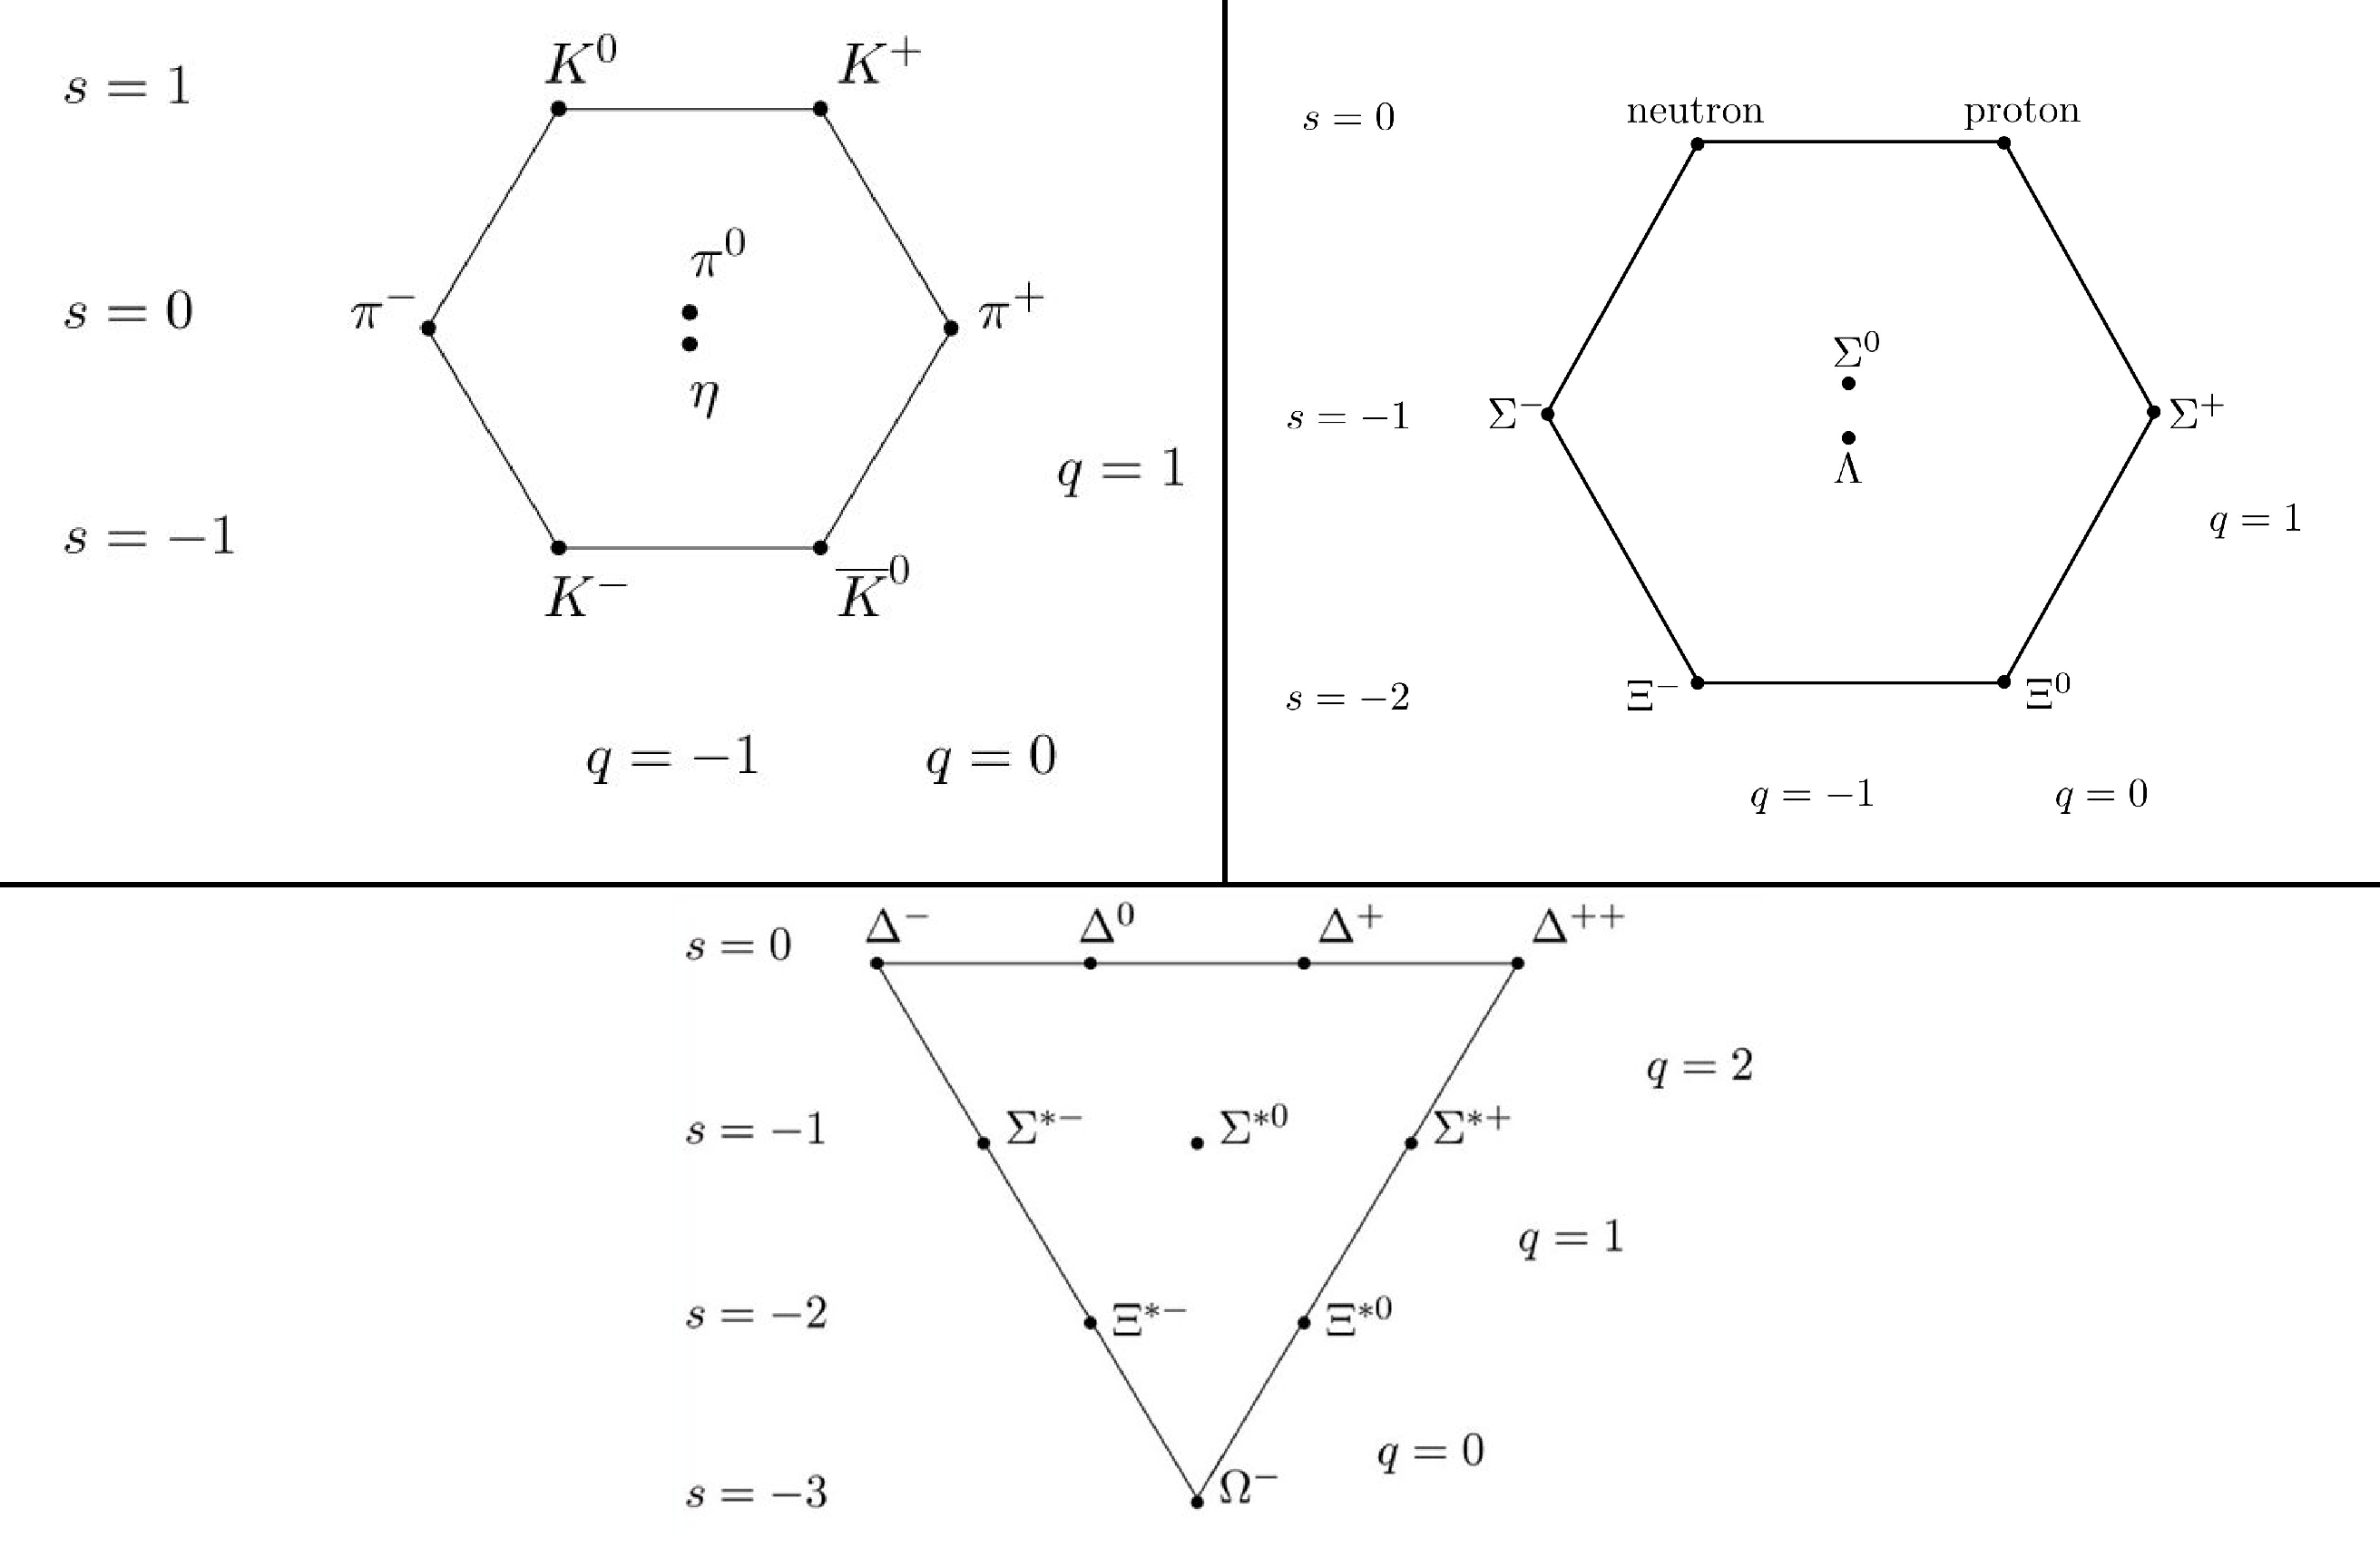
\includegraphics[width=5in]{figures/background/mesons_baryons.pdf}
	\caption{The octets and decuplet of Gell-Mann's ``Eightfold Way''. Top left: the eight particles of the meson octet; top right: the spin-$\frac{1}{2}$ baryon octet; bottom: the spin-$\frac{3}{2}$ baryon decuplet.}
	\label{fig:mesons-baryons}
\end{figure}

Near the end of the 1960's, SLAC began the first set of experiments to use an electron beam to investigate the nucleon in what is now known as Deep Inelastic Scattering (DIS). What they discovered was that the functions used to describe nuclear structure were largely independent of momentum transfer ($Q^2$) above a certain threshold. This so-called ``scaling'' behavior lent credence to the theory that nucleons were composed of a point-like particles. This discovery coupled with the proliferation of new particles (the ``particle zoo'') led Murray Gell-Mann and Yuval Ne'eman to construct a framework that would make some sense of it all. Gell-Mann had organized the host of mesons and baryons discovered into a geometric order named the ``Eightfold Way''\footnote{Gell-Mann here makes a rather poetic allusion to the Buddhist ``Noble Eightfold Path''} as depicted in Figure~\ref{fig:mesons-baryons}. The underlying explanation for all of this, as described independently by Gell-Man and Ne'eman, was to characterize these many particles as the several combinations of three \emph{flavors} of constituent particles, named \emph{quarks}~\cite{joyce1999finnegans}. The flavors, \emph{u}, \emph{d}, and \emph{s} were named \emph{up}, \emph{down}, and \emph{strange}. Here, mesons were predicted to be composite particles of integer spin containing two quarks and baryons be half-integer spin particles composed of three quarks. This model led Gell-Mann to predict the existence of the $\Omega^-$ particle, along with its \emph{strangeness}, charge, and mass. The discovery of this particle\cite{1964PhRvL:12204B} earned Gell-Mann the 1969 Nobel Prize for his work on the quark model.

Though this model was a breakthrough in the understanding of fundamental particles, it did not comprehensively describe all experimental data. For example, when accounting for the total momentum of a nucleon, it was found that only $\sim50\%$ of the momentum was being carried by the quarks. It was not until the theory of quantum chromodynamics (QCD) came along that this and several other mysteries could be explained. QCD described the mechanism of a 3-fold \emph{color} charge and the gauge bosons, gluons, that intermediate the strong force between quarks (and other gluons). In the particular case of the missing momentum, this was found to reside in the intermediating gluons\cite{PhysRevLett.43.830}, which carry only color charge, to which the electro-weak probes used were insensitive.

Many nuclear probes and methods have been used to characterize the distributions and characteristics of nuclear partons, including the aforementioned DIS process. As I will describe later in this section, much has been learned about parton probability distribution functions with this and other processes, but it is the process of hadron-hadron di-lepton production that is of primary focus in this paper, which allows for an alternative approach to investigate the structure and characteristics of the quarks inside of a nucleon, and perhaps shed some light on some ongoing mysteries in nuclear physics.

\section{Di-lepton production in nucleon-nucleon collisions}

Studying the production of pairs of leptons resulting from hadron-hadron collisions has proven to be a powerful tool in probing nucleon structure and parton distribution functions (PDFs). Figure \ref{fig:DY-spectrum} shows the mass spectrum of the muon mode of di-lepton production in proton-nucleus collisions measured at the E-866/NuSea experiment at Fermilab\cite{PhysRevLett.80.3715}. The resonances of the $J/\Psi$, $\Psi^\prime$, $\Upsilon$, $\Upsilon^\prime$, and $\Upsilon^{\prime\prime}$ can be seen atop a smooth, continuous distribution which decreases with mass. The process responsible with this distribution of $\mu^+\mu^-$ pairs is the Drell-Yan process\cite{PhysRevLett.25.316}, which is illustrated in the Feynman diagram in Fig.~\ref{fig:dy-diagram}. This process is characterized by a quark annihilating with an anti-quark to form a virtual time-like photon which then decays into a pair of leptons. The study of this process can lend some insight into nucleon structure due to the fact that the mass and momentum of the di-lepton pair directly reflects the momentum distributions of the interacting quarks and anti-quarks. Current knowledge and models\CN of these momentum distributions come primarily from deep-inelastic lepton scattering (DIS) and the Drell-Yan (DY) process.

\begin{figure}
	\centering
	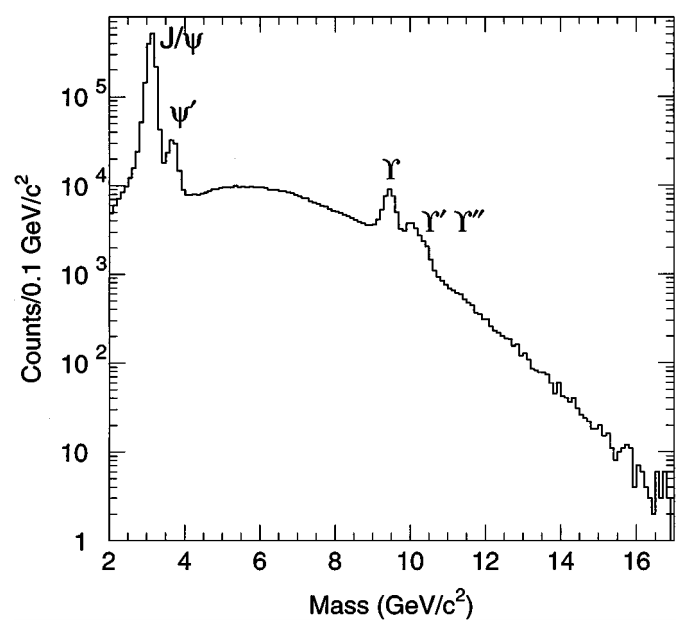
\includegraphics[width=3in]{figures/background/DY-spectrum-e866.png}
	\caption{Dimuon mass spectrum from E-866 $p+h$ collisions at \unit[800]{GeV/c}\cite{PhysRevLett.80.3715}.}
	\label{fig:DY-spectrum}
\end{figure}

%Di-lepton production has a record of being used as a technique for searching for new particles. 
One particular focus of study for the Drell-Yan process is its nucleon number-dependent (A-dependent) behavior of its cross sections. This is of particular interest due to a phenomenon known as the EMC effect, in which the European Muon Collaboration (EMC) discovered in 1983 that parton distribution functions become modified when in the presence of the nuclear medium. This A-dependent behavior was not expected for hard scattering processes as the modest (maximum $\unit[8.8]{MeV}$) binding energy of a nucleus on a nucleon was not thought to have a significant effect on quark momentum distributions within a nucleon (\unit[938]{$Mev/c^2$}). Many experiments since\CN have confirmed, extended, and precisely characterized the A-dependent behavior observed. Among the many hard scattering probes for investigating this phenomenon, the Drell-Yan process is uniquely capable of isolating the effect on the anti-quark distributions to a high degree of accuracy. The study of the effects of the nuclear medium on nucleon anti-quark distributions is the secondary research goal of the SeaQuest experiment and is the main focus of this thesis.

Within this thesis, the Drell-Yan process and its properties are discussed in \red{sections so and so} and various A-dependent behaviors seen in Drell-Yan and DIS are discussed in \red{sections so and so}. A few models are discussed in an attempt to theoretically characterize this A-dependent behavior in \red{sections so and so}.

In cases where a Drell-Yan process occurs, it can often be the case that the incident quark must pass through the strongly-interacting nuclear medium prior to its annihilation with the anti-quark in the target. By investigating the momentum distribution of the quark from the beam and it's A-dependence, some insight can be gained regarding the parton energy loss as it moves through a foreign nuclear medium. This topic and its existing data are briefly discussed in \red{section so and so}.

\subsection{The Drell-Yan Process}

\begin{figure}[h]
	\centering
	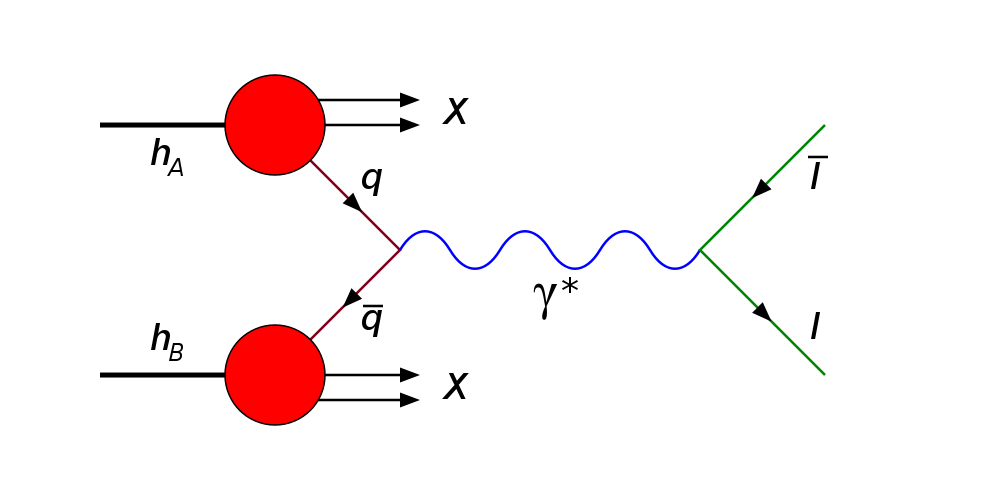
\includegraphics[width=4.5in]{figures/background/Drell-Yan.png}
	\caption{The Drell-Yan process, an $s$ channel interaction consisting of the annihilation of a quark with an anti-quark.}
	\label{fig:dy-diagram}
\end{figure}

The study of continuum di-lepton production in hadron collisions,
\begin{equation}
	h_A +  h_B \rightarrow l^+ l^- + X
	\label{eq:hh2ll}
\end{equation} 
can be used to study hadronic structure in a way that is complementary to the study of deep-inelastic scattering,
\begin{equation}
l + h \rightarrow l^\prime + X.
\label{eq:lh2lx}
\end{equation}
In 1970, S. Drell and T.M. Yan were the first to suggest that, at high $Q^2 (=M^2_{l^+ l^-}) \geq 16GeV^2$, the quarks inside the hadrons $h_A$ and $h_B$ can be considered free fermions in the instantaneous moment that they interact. The Drell-Yan model addresses the dominant subprocess here,
\begin{equation}
q_A + \bar{q}_B \rightarrow \gamma^* \rightarrow l^+ l^-
\label{eq:dy-process}
\end{equation} 
as an electromagnetic annihilation process. In this high-$Q^2$ kinematic space, the final state of the hadrons that contain these quarks becomes irrelevant. By the energy-time uncertainty principle\CN of $\Delta E \Delta t \sim \hbar$, the timescales under consideration are $<10^{-25}s$, and the corresponding distances are $<10^{-17}m$, where the size of a nucleon is $\sim 10^{-15}m$\CN. At these short space-time scales, electromagnetic annihilation dominates this quark-quark interaction.

This is further reinforced by the widely accepted non-Abelian gauge field theory of Quantum Chromodynamics (QCD) which describes the interactions between quarks and gluons. QCD provides a theoretical justification for treating Drell-Yan processes as events isolated from the rest of the hadron states, and it does so through the concept of the running of the coupling constant, or \emph{asymptotic freedom}\cite{Bethke:2006ac}. This characteristic feature of QCD is described by the decrease of the strength of the strong force coupling constant as the space-time scale of the interaction approaches zero (i.e. as $Q^2 \rightarrow \infty$). The strong coupling constant can be expressed as a function of $Q^2$:
\begin{equation}
\alpha_s(Q^2) = \frac{1}{\beta_0 \ln (Q^2/\Lambda^2)}
\end{equation}
where
\begin{equation}
\beta_0 = \frac{12\pi}{33-n_f}
\end{equation}
Here, $\Lambda$ is the QCD scale parameter that depends on the number of quark flavors, $n_f$, and the renormalization scheme, measured to be around $\sim$ \unit[217]{MeV}. Experimental measurements of the running of the coupling constant as measured by many different processes can be seen in Figure~\ref{fig:asymptotic-freedom}.
\begin{figure}
	\centering
	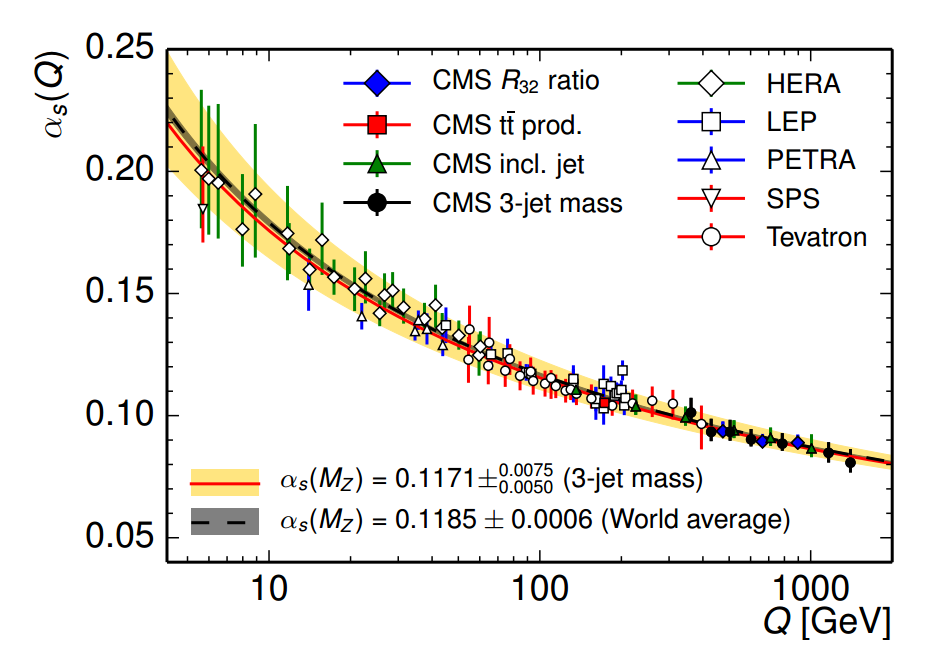
\includegraphics[height=3in]{figures/background/running-strong-coupling.png}
	\caption{A compilation of measurements of the running of the strong coupling constant, $\alpha_s(Q^2)$\cite{CMS:2014mna}.}
	\label{fig:asymptotic-freedom}
\end{figure}

It is useful to have some intuition as to the reason for these ``running'' of the coupling constants. The phenomenons responsible are termed ``screening'' and ``anti-screening'' (or ``camouflaging'')\cite{Quigg:1985ai}. This straightforward in the case of the electromagnetic force which can be seen depicted in the left pane of Figure~\ref{fig:screening-camo}. Whether it is in some kind of dielectric medium or in an isolated vacuum (where quantum fluctuations lead to virtual $e^+e^-$ pairs), the charges surrounding an individual charged particle are oriented in such a way as to decrease the overall observed charge. In the realm of QED, the higher energies you use to probe a particle, the closer you actually get to seeing the ``actual'' charge of the particle, and as such, the EM coupling constant increases at higher energies.

The same is seen in the case of QCD with its non-binary charge scheme. It's more difficult to conceptualize, but the same screening effect exists in the case of a particle with color charge. The middle pane of Fig.~\ref{fig:screening-camo} is a depiction of screening analogous to the familiar EM screening. The difference between QCD and QED with the behavior of the coupling constants is attributable to the fact that the force-carrying boson of QCD, the gluon, carries with it its own color charge. In the QED picture, the charge at the center is continuously emitting and absorbing photons as it interacts with the surrounding charges, but its charge does not change. With the color-charged particle, gluons are also being continuously emitted and absorbed, but an effect of that is a change in color charge. The result ends up being the phenomenon of camouflaging where, the closer you are to a color-charged particle, the less that you can ``see'' the \emph{net} charge, and the actual charge of the particle is obfuscated. The net charge of the particle, statistically, becomes neutral, causing the strong force to become increasingly feeble at smaller scales (compared to the strength of QED interactions). This effect competes with and surpasses the color screening that occurs and is the root cause of the asymptotic freedom in QCD. On the flip side, the farther you get from the color charge, the more you are exposed to the full true net charge, and the stronger the coupling becomes. This increase in the coupling is the QCD confinement that is observed. An example if in the right pane of Fig.~\ref{fig:screening-camo} where the quark emits many gluons, thus changing its color from Blue to Green, but when summing over all colors emitted and absorbed, the net color is still Blue.

\begin{figure}
	\centering
	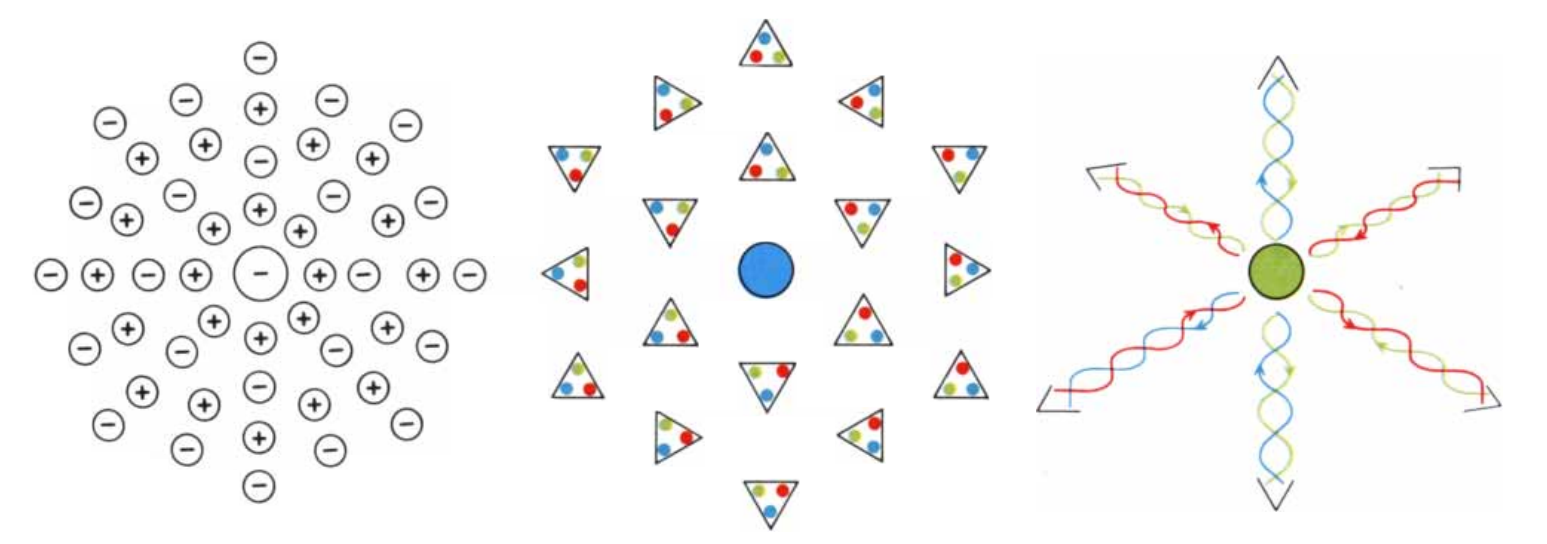
\includegraphics[width=\textwidth]{figures/background/screening-camo.png}
	\caption{(Left) classic electromagnetic screening of a free charge in a dielectric or even a vacuum. (Center) The analogous screening in the three-charge QCD regime. (Right) The color camouflaging due to the constant absorption/emission of colored gluons\cite{Quigg:1985ai}.}
	\label{fig:screening-camo}
\end{figure}

\subsection{Drell-Yan Kinematics}

In the center-of-mass frame, the Drell-Yan process can be broken down into three stages with three sets of kinematics (refer to Fig.~\ref{fig:dy-diagram}). Beginning with the quarks, \emph{x} is defined as the fraction of the hadron's momentum carried by the interacting quark or antiquark. Conventionally in fixed-target experiments, subscripts are assigned as $x_1$ and $x_2$, which refer to the quark/antiquark from the beam and the antiquark/quark from the target, respectively. This \emph{x} is called the Bjorken \emph{x}, and is well-known in DIS processes to have a value of
\begin{equation}
x = -q^2/2 p \cdot q
\end{equation} where \emph{p} and \emph{q} are the 4-momenta of the hadron and the photon. In DY, the same momentum fraction $x$ is used to describe part of the fundamental basis of the interaction. In this case, $q$ is the 4-momentum of the virtual photon and $p$ is the 4-momentum of the hadron that contains the quark in question.

The next stage of the process is the virtual photon. This photon' properties are effectively equivalent to the `dimuon' or `dilepton', which are the terms more commonly used in referring to kinematics. The first of its relevant kinematics is its mass $M_{\gamma^*}$, which represents its energy and virtuality. The value $x_F$, or Feynman-x, is the fraction of the maximum possible longitudinal momentum carried by the virtual photon in the beam direction. The transverse momentum, $p_T$, and the azimuthal production angle, $\phi_{\gamma^*}$ are the remaining kinematics associated with the virtual photon.

\red{Get solid intuition for different CS angles.}

The third stage regards the pair of leptons produced. In the frame of the virtual photon, there is a polar and azimuthal decay angle, $\theta_\mu$ and $\phi_\mu$, respectively, for each of the decay muons. It becomes impossible, however, to reconstruct these variables, as the individual transverse momenta of the quarks are unknown, and the thus the quark-antiquark annihilation axis is unknown. This is remedied by shifting the process into the Collins-Soper (CS) reference frame\cite{PhysRevD.16.2219} which orients the reference axis to be parallel to the bisector of the angle between the interacting hadrons in the rest frame of the muon pair. A depiction of the Collins-Soper frame can be found in Fig.~\ref{fig:collins-soper}. In total, this brings a total of eight kinematic variables, summarized in Table~\ref{tab:var}.
\begin{figure}
	\centering
	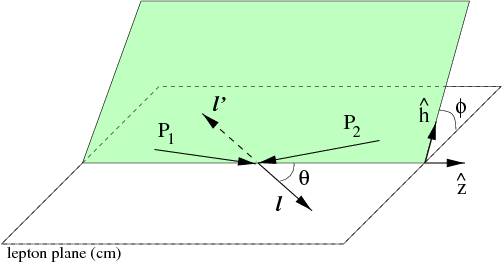
\includegraphics[width=4.50in]{figures/background/collins-soper.png}
	\caption{A depiction of the Collins-Soper reference frame. The green plane along $\hat{h}$ is the plane shared by the two hadrons.}
	\label{fig:collins-soper}
\end{figure}

Experimentally, six independent variables are measured, which form a basis by which all eight can be known. This is due to the fact that two pairs of variables, ($M_{\gamma^*}$, $x_F$) and ($x_1$, $x_2$) are correlated by the following, ignoring quark masses and considering $p_\perp << p_{\ell}$:
\begin{eqnarray}
x_F & \equiv & \frac{p_{\ell}}{\sqrt{s}/2} \approx x_1 - x_2 \label{eq:xf=x1-x2} \\
M_{\gamma^*}^2 & \equiv & E^2 - p_{\ell}^2  = s x_1 x_2 \label{eq:m=sx1x2} \\
E & = & \frac{1}{2}(x_1 + x_2) \sqrt{s} \\
p_{\ell} & = & \frac{1}{2}(x_1 - x_2)\sqrt{s}
\end{eqnarray}
In this frame, the longitudinal momenta of the quarks are $x_1 \sqrt{s}/2$ and $- x_2 \sqrt{s}/2$, with $\sqrt{s}$ being the center of mass energy of the hadronic collision. So, by measuring the 3-momenta of the $\mu^+$ and $\mu^-$, the quantities ($M_{\gamma^*}$, $x_F$, $p_T$, $\phi_{\gamma^*}$, $\theta_\mu$, $\phi_\mu$), which is sufficient to calculate the remaining ($x_1, x_2$) in our approximation.

\begin{table}[h]
	\centering
	\begin{tabular}{c|r}
		Variable&Description\\ \hline \hline
		$x_{1/2}$ & Momentum fraction of the beam/target quark\\
		$M_{\gamma^*}$ & Mass of the virtual photon (dimuon)\\
		$x_F$ & Fraction of the max. possible $p_{\ell}$ carried by virt. photon\\
		$p_T$ & Transverse momentum carried by the virt. photon\\
		$\theta_{\mu}, \phi_{\mu}$ & Polar and azimuthal decay angle\\ & of one of the muons, in the CS ref. frame\\ \hline
		$\alpha$ & The fine structure constant \\
		$K(x_1,x_2)$ & High-order QCD correction term \\
		$\sqrt{s}$ & Center of mass energy of the hadronic collision \\
		$\sqrt{\hat{s}}$ & Center of mass energy of the $q\bar{q}$ collision \\
		$Q^{2}$ & Four-momentum of the intermediate time-like photon, squared \\ 
		$q_i^{t/b}(x)$ & The quark number density in the nucleon of the target/beam \\ \hline \hline
	\end{tabular}
	\caption{Kinematic variables relevant to the Drell-Yan process .}
	\label{tab:var}
\end{table}

\subsection{Cross-Section}

As the participating quarks are asymptotically free within each hadron, there will be no correlations between the probability distributions of the annihilating particles, and the process is independent of the distributions. As a result, the cross section of the Drell-Yan process can be reduced to a function of the electromagnetic annihilation process and the quark probability distribution functions. With these components and some QCD considerations, we can construct it piece by piece.

The first step is to begin with the known hard scattering cross section of $\epsilon + \bar{\epsilon} \rightarrow l^+ l^-$, where $\epsilon$ is an arbitrary particle. This cross section\cite{Halzen:1984mc} is given by
\begin{equation}
\sigma(\epsilon\bar{\epsilon}\rightarrow l^+l^-) = \frac{4 \pi \alpha^2}{3M_{\gamma^*}^2} e_f^2
\label{eq:annihilation-cross}
\end{equation}
where $\alpha$ is the electromagnetic fine structure constant, $e_f$ is the charge of the particle, and $M_{\gamma^*}$ is the dilepton mass. With this, we add the QCD consideration that only $q\bar{q}$ of opposite color can annihilate with each other into a colorless virtual photon. Possible combinations are $R\bar{R}$, $B\bar{B}$, and $G\bar{G}$ out of $3\times 3$ possible cases. As such, an overall factor of $\frac{1}{3}$ is added to this cross section. Finally, factoring in the conservation of flavor (there can only be $u\bar{u}$, $d\bar{d}$, etc. combinations) and the quark structure of hadrons A and B,  we use the product ($q_f^A(x_1)\bar{q}_{f}^B(x_2)$) of the quark probability distributions for finding quarks of the same flavor-antiflavor combination in the two hadrons. It must also be considered that the quark or antiquark may be found in either hadron A or hadron B. The product of these three factors leads us to the Drell-Yan cross section\cite{Drell:1970wh}
\begin{eqnarray}
\frac{d^2\sigma}{dx_1dx_2}&=&\frac{1}{3}\frac{4\pi\alpha^2}{3M_{\gamma^*}^2}
\sum_{f}e_f^2[q_f^A(x_1)\bar{q}_f^B(x_2)+
\bar{q}_f^A(x_1)q_f^B(x_2)]\\
&=&\frac{4\pi\alpha^2}{9 s x_1 x_2}
\sum_{f}e_f^2[q_f^A(x_1)\bar{q}_f^B(x_2)+
\bar{q}_f^A(x_1)q_f^B(x_2)]
\label{eq:DY-cross}
\end{eqnarray}
where the sum is summing over flavors of quarks ($f\in\{u,d,s,...\}$). This can be evaluated in terms of the measurables $M_{\gamma^*}$ and $x_F$ via Equations~\ref{eq:xf=x1-x2}~and~\ref{eq:m=sx1x2}
\begin{equation}
M_{\gamma^*}^2 \frac{d^2\sigma}{dM_{\gamma^*}^2 dx_F} = 
\frac{1}{3}\frac{4\pi\alpha^2}{3M_{\gamma^*}^2}
\frac{x_1 x_2}{x_1 + x_2}
\sum_{f}e_f^2[q_f^A(x_1)\bar{q}_f^B(x_2)+
\bar{q}_f^A(x_1)q_f^B(x_2)]
\label{eq:dy-cs-observe}
\end{equation}
where $x_1$ and $x_2$ can be expressed as
\begin{equation}
x_1 = \frac{1}{2}\left[\sqrt{x_F^2 + 4\tau} + x_F\right],\ \  
x_2 = \frac{1}{2}\left[\sqrt{x_F^2 + 4\tau} - x_F\right],\ \ 
\tau = \frac{M_{\gamma^*}^2}{s}
\end{equation}
The cross section can also be represented by dimensionless variables in its scaling form,
\begin{equation}
s \frac{d^2\sigma}{d \sqrt{\tau} dy} = 
\frac{1}{3}\frac{4\pi\alpha^2}{3}
\sum_{f}e_f^2[q_f^A(x_1)\bar{q}_f^B(x_2)+
\bar{q}_f^A(x_1)q_f^B(x_2)]
\label{eq:dy-cs-dimensionless}
\end{equation}
where we introduce the rapidity term $y$ in describing $x_1$ and $x_2$,
\begin{equation}
y  = \frac{1}{2} \ln \frac{E+ p_\ell}{E-p_\ell} = \frac{1}{2} \ln \frac{x_1}{x_2},\ \ 
x_1  = \sqrt{\tau} e^{y},\ \  
x_2  = \sqrt{\tau} e^{-y}
\end{equation}
It should be noted that with collider experiments, it is conventional to refer to the hadrons A and B in terms of the beam and target hadrons, respectively, and as such, $x_1$ refers to the the quark in the beam hadron and $x_2$ refers to the quark in the target hadron.

In each of these equations~\ref{eq:DY-cross}, \ref{eq:dy-cs-observe}, and \ref{eq:dy-cs-dimensionless}, the cross sections can be factored into two parts: one subprocess cross section and one part that has only a dependence on the parton distribution functions. They are independent of each other, because one of the staples of the quark parton model is that the PDFs ($q(x)$ and $\bar{q}(x)$) are independent of the process by which they are probed. This feature is commonly referred to as the ``universality'' of the PDFs.

\section{Nucleon Structure}

\subsection{PDFs, Structure Functions, and the Quark Parton Model}

\red{Mention TMDs and spin structure functions more.}

In the context of hadron-hadron collisions, one can interpret the PDFs as follows: consider two hadrons A and B colliding; a parton of type \emph{a} ($a\in \{u, d, s, g, ...\}$) comes from A and carries with it a fraction of A's momentum ($x_A$).  The same goes for hadron B; a parton of type \emph{b} comes from B and carries momentum fraction $x_B$. Now, the probability of finding the discussed parton from A at momentum fraction $x_A$ is given by $q_{a/A}(x_A)$. Likewise, the probability of finding the discussed parton from B at $x_B$ is $q_{b/B}(x_B)$.

In general, experimental data measuring $F_2$ is used in conjunction with some general constraints in order to arrive at the calculated PDFs. One constraint is to consider the known number of valence quarks in a nucleon. Since the function $q_f(x)$ can be interpreted to be the number density of quark flavor $f$ as a function of momentum fraction $x$, the value $q_f(x)dx$ represents the number of quarks with flavor $f$ with fractional momentum in the range of $[x,x+dx]$. Therefore, the known number of valence quarks of flavor $f$ ($N_f$) provides the following condition.
\begin{equation}
\int_0^1 dx [q_f(x) - \bar{q}_f(x)] = N_{f}
\label{eq:vsr}
\end{equation}
Another condition considers the value $x q(x) dx$, which is the total momentum fraction of the hadron of the number of quarks $q(x)dx$. This provides a logical constraint is the summation of the momentum fractions of all partons must add up to the full nucleon momentum:
\begin{equation}
\sum_{q,\bar{q},g} \int_0^1 dx [x q(x)] = 1
\end{equation}
It should also be noted that the quark PDFs can be split with respect to their spin alignment ($+$) or anti-alignment ($-$) with the nucleon's spin
\begin{equation}
q(x) = q^+(x) + q^-(x)
\end{equation}
and the polarized (or helicity) PDF can be defined as
\begin{equation}
\Delta q(x) = q^+(x) - q^-(x)
\end{equation}
though, due to the fact that SeaQuest uses neither a polarized $\Delta q(x)$. There are two standing proposals, however, to extend the SeaQuest spectrometer for an additional period of data taking, augmenting it with a polarized proton beam (FNAL E-1027) and/or a polarized target (FNAL E-1039). The polarized beam proposal adds two beam-polarizing apparatuses named \emph{Siberian Snakes} to provide sufficiently polarized protons. The polarized target modification calls for the construction and installation of a new cryogenic liquid target system. Both proposals have been approved by the FNAL review committee and are likely to be acted upon near the end of the E-906 contract.

The structure functions $F_1, F_2,$ and $g_1$ of the nucleon are interpreted in the QPM as the charge-weighted sums over the quark flavors of the corresponding PDFs:
\begin{eqnarray}
F_1(x) = \frac{1}{2} \sum\limits_f e_f^2 q_f(x) \label{eq:f1} \\
F_2(x) = \sum\limits_f e_f^2 x q_f(x) \label{eq:callan-gross} \label{eq:f2} \\
g_1(x) = \frac{1}{2} \sum\limits_f e_f^2 \Delta q_f(x) \label{eq:g1}
\end{eqnarray}
where here $f$ represents all flavors of of quarks and anti-quarks. We see above the relation between $F_1(x)$ and $F_2(x)$ known as the Callan-Gross relation ($F_2 = 2xF_1$). This relation relies on the partons having spin-$\frac{1}{2}$ and no transverse momentum in the infinite momentum frame. The full expression is
\begin{equation}
F_2 = 2xF_1 \frac{1 + R}{1 + 2 M_N x/\nu}
\end{equation}
where $M_N$ is the nucleon mass and $R=\sigma_L/\sigma_T$ is the ratio of cross sections for absorbing a longitudinal to that for a transverse photon. Experimentally, R is small\cite{PhysRevLett.61.1061} ($\lesssim0.1$) for $x\gtrsim0.1$ and for $Q^2\gtrsim$\unit[5]{GeV$^2$}. Also, when assuming the infinite momentum frame, $\nu$, the energy transferred by the photon is assumed to trend towards infinity. As a result, this relation reduces to the commonly-used Callan-Gross relation.

Due to the complex nature of lattice QCD\footnote{An approach to solving quantum chromodynamics situations by simulating quarks and gluons on a set of lattice points in spacetime and modeling their well-defined interactions.} simulations, the parton distributions $q_f(x)$ and $\bar{q}_f(x)$ within the nucleus are determined empirically, with only a few rules based in theory. The primary probe used to measure them has been deep inelastic scattering (DIS), examining the inclusive jet production in order to get a clearer picture of nucleon structure. Data from many different experiments are combined  to extract the unpolarized PDFs. The earlier parametrizations of the PDFs first relied on fits to the measured structure functions solely from DIS experiments which are primarily sensitive to the light quark distributions and are unable to disinguish between quarks and antiquarks of the same flavor. More modern parametrizations use many different processes to extract supplementary and complementary information that can be incorporated. Lepton-charge asymmetry observed in $W^\pm$ production provides additional light quark distribution information. Jet production and photon measurements are also used to set constraints on gluon distributions. It should be noted that Drell-Yan dilepton production from such experiments as E605 and E866 that have contributed constraints on the light anti-quark distributions from the nucleon sea.

The current status of the experimental determination of these PDFs is led by CTEQ (Coordinated Theoretical-Experimental Project on QCD) and TEA (\red{which stands for???}), and are illustrated in Figures~\ref{fig:pdf-q2}~and~\ref{fig:pdf-q100}. The CTEQ-TEA calculated these PDFs from data on inclusive, high-momentum transfer processes, for which perturbative QCD is expected to be reliable. In the case of deep inelastic lepton scattering, only data with $Q > 2$ GeV is used. Data in this region are expected to be relatively free of non-perturbative effects, such as higher twists or nuclear corrections. Thus, there is no need to introduce phenomenological models for nonperturbative corrections beyond the leading-twist perturbative contributions\cite{Dulat:2015mca}.

\begin{figure}
	\centering
	\subfloat[][PDFs $x f_q(x, Q)$ for Q=2 GeV.]{%
		\label{fig:pdf-q2}%
		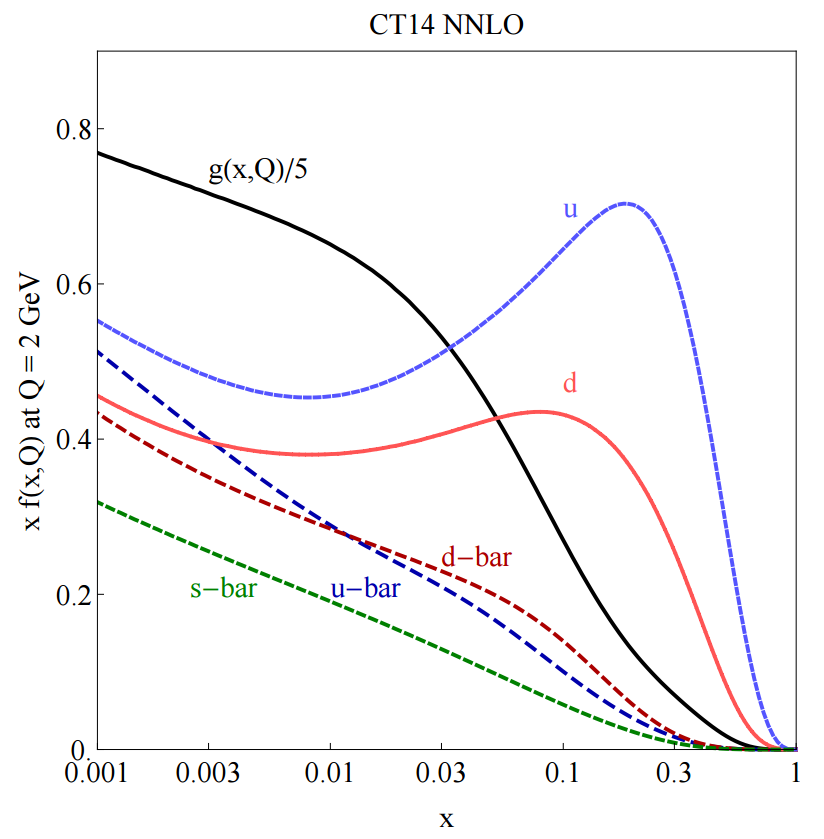
\includegraphics[width=0.45\linewidth]{figures/background/parton-dist-q2.png}}
	\hspace{8pt}%
	\subfloat[][PDFs of $x f_q(x, Q)$ for Q=100 GeV.]{%
		\label{fig:pdf-q100}%
		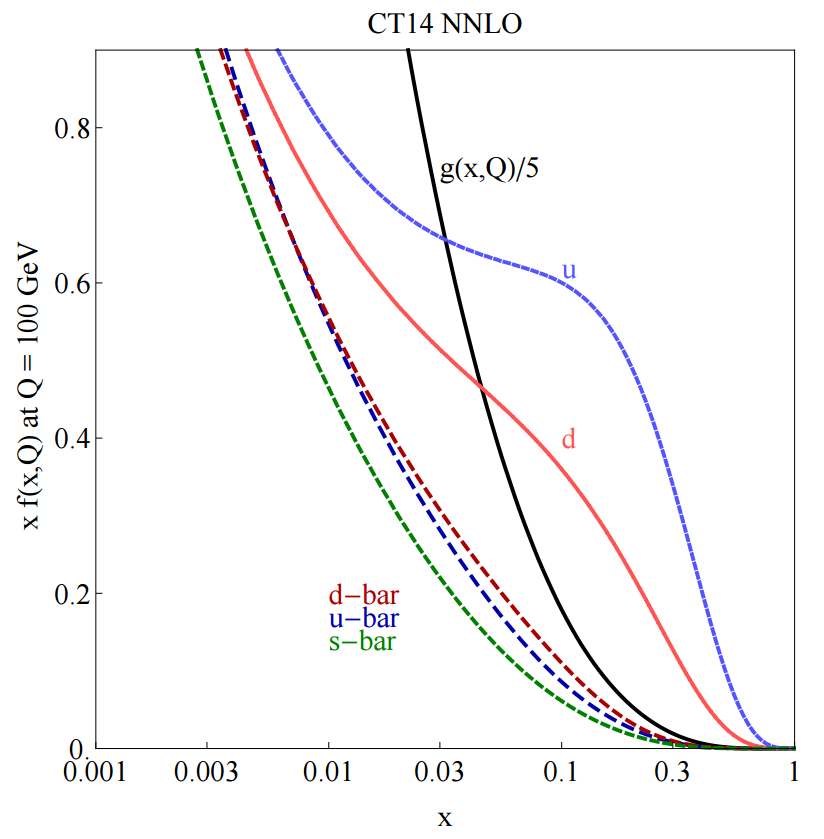
\includegraphics[width=0.45\linewidth]{figures/background/parton-dist-q100.png}}
	\caption{Parton distribution functions for quarks and gluons and their \emph{x} and \emph{Q} dependence as calculated to NNLO by the CTEQ-TEA (CT) global analysis group\cite{Dulat:2015mca}.}
	\label{fig:pdf-q2-q100}
\end{figure}

Looking to Figure~\ref{fig:pdf-q2-q100} we see that at $x>0.1$, $u$ and $d$ quarks dominate $\bar{u}$ and $\bar{d}$ quarks. The SeaQuest spectrometer (described in detail in the next chapter) is a ``forward spectrometer'', which means that, for PDF-relevant purposes, the high-$x_F$ ($x_F>0$) kinematic phase space is explored, which translates to high $x_1$ and low $x_2$. With this consideration, the Drell-Yan process measured at SeaQuest is probabilistically dominated by a quark from the beam annihilating with an anti-quark from the target. Further, all anti-quarks that exist in the target nucleons must come from what are called the \emph{sea quarks}, or the virtual $q\bar{q}$ pairs 
that arise from gluons splitting. 

Other interesting observations and measurements that have gone into these distributions are the observations of momentum contributions from all quarks and antiquarks and the momentum fraction from just antiquarks. The momentum sum
\begin{equation}
x_{tot} = \int_0^1 dx [F_2(x)] \simeq \int_0^1 dx [x(q(x) + \bar{q}(x))] \label{eq:mom-sum}
\end{equation}
showed that $x_{tot}$ for quarks is $0.512 \pm 0.018$\CN. The rest was found to be attributed to the gluons, though they could not be detected directly by an electron beam in DIS since they carry no electric charge. The momentum fraction from just anti-quarks comes from clever use of another structure function, $F_3$.
\begin{eqnarray}
F_3^{\nu N}(x) & = & q(x) - \bar{q}(x) - 2s(x) + 2c(x) \\
F_3^{\bar{\nu} N}(x) & = & q(x) - \bar{q}(x) + 2s(x) - 2c(x) \\
F_3(x) & = & \frac{1}{2} [F_3^{\nu N}(x) + F_3^{\bar{\nu} N}(x)] = q(x) - \bar{q}(x) = u_v(x) + d_v(x)
\end{eqnarray}
Here, the $v$ subscript denotes valence quark distributions, $q/\bar{q}(x)$ are
\begin{eqnarray}
q(x) & = & u(x) + d(x) + s(x) + c(x) \\
\bar{q}(x) & = & \bar{u}(x) + \bar{d}(x) + \bar{s}(x) + \bar{c}(x)
\end{eqnarray}
and the individual $F_3^{\nu/\bar{\nu}N}$ structure functions are measured from $\nu N$ and $\bar{\nu} N$ scattering and then combined\CN. With $F_3$, there is the Gross-Llewellyn Smith (GSL) sum rule\cite{Gross:1969jf}
\begin{equation}
\int_0^1 F_3(x) = 3
\end{equation}
which is to say that there are three valence quarks. The new information gained here with $F_3$ though is the measurement of $\int dx [xF_3(x)] = 0.341 \pm 0.036$, which gives the momentum fraction carried by the valence quarks. Put this together with the results of Eq.~\ref{eq:mom-sum} and one can derive the conclusion that the anti-quarks in the nucleon possess between 13\% and 17\% of the nucleon's momentum\cite{Fisk:1982pn}.

The last interesting sum rule to discuss is the Gottfried sum rule which is focused on flavor asymmetries between the proton and its isospin partner, the neutron.
\begin{eqnarray}
  S_G & = & \int_0^1 dx \left[\frac{F_2^p - F_2^n}{x}\right] \\
  & = & \int_0^1 dx \left[ \sum\limits_f e_f^2 [q_f^p(x) + \bar{q}_f^p(x) - q_f^n(x) - \bar{q}_f^n(x)] \right]
\end{eqnarray}
We assume charge symmetry insofar as $u^p(x) = d^n(x)$ and $\bar{u}^n (x) = \bar{d}^p(x)$, yielding
\begin{equation}
S_G = \int_0^1 dx \left[ \frac{1}{3} (u(x) + \bar{u}(x) - d(x) - \bar{d}(x)) \right]
\end{equation}
where these PDFs refer to the distributions in the proton. By some reorganization and grouping, this can be re-expressed in a more familiar way.
\begin{equation}
S_G = \int_0^1 dx \left[\frac{1}{3} [u(x) - \bar{u}(x)] \right] - 
      \int_0^1 dx \left[\frac{1}{3} [d(x) - \bar{d}(x)] \right] -
      \int_0^1 dx \left[\frac{2}{3} [\bar{d}(x) - \bar{u}(x)] \right]
\end{equation}
The first two integrals here are the definitions of the valence quark sum rule mentioned in Eq.~\ref{eq:vsr}, and this is known to be 2 and 1 for the $u$ and $d$ valence quarks of the proton, respectively. As a result, we arrive at the common representation of the Gottfried Sum Rule (GSR).
\begin{equation}
	  S_G = \frac{1}{3} - \int_0^1 dx \left[ \frac{2}{3} [\bar{d}(x) - \bar{u}(x)] \right]
      \label{eq:gsr}
\end{equation}
If one were to assume that, within a proton, $\int dx [\bar{u}(x)] = \int dx[\bar{d}(x)]$, then this sum reduces to $\frac{1}{3}$. More on this sum and its measured violation in a later section.

\subsection{Drell-Yan Tests of the QPM}

The Drell-Yan process can be described within the frameworks of QPM and QCD, so it provides a good testing ground for these models. Even further, the very clean leptonic DY signature offers a good vantage point by which to confirm the parton picture experimentally. The testing process begins with establishing the validity of the quark-parton model via Drell-Yan. Once this is done, the following step would be to study the deviation between measurements and what is expected.

\subsubsection{Quark charge}

\subsubsection{Spin-1/2 quarks and the Lam-Tung Relation}


\subsubsection{Transverse momentum}


\subsubsection{Point-like quarks}

If the quarks in the QPM are point-like and without any substructure, then the DY cross section (expressed in Eq.~\ref{eq:dy-cs-dimensionless}) across $Q^2$ ($\sqrt{s}$) should exhibit scaling behavior 

\red{\begin{itemize}
		\item Point-like quarks
		\item quark charge
		\item quark spin
		\item end with departure of Drell-Yan from QPM with scaling violation and the magnitude of DY over prediction (K-Factor), and pT
	\end{itemize}}

\subsection{QCD-Improved Drell-Yan}

\red{\begin{itemize}
		\item Gluon interactions complicate the na\"{i}ve DY picture,
		\item Describe QCD corrective processes
		\item Maybe move $\alpha_s$ and running of coupling constant to here
		\item Introduce Q-dependence of PDFs
		\item QCD calculation of K-factor
		\item Transverse momentum in QCD picture
	\end{itemize}
}
%In addition to the leading-order DY term, there are high-order QCD corrections to consider. These have been studied and accounted for up to $\bigoh(\alpha_s)$ and $\bigoh(\alpha_s^2)$. These include contributions from high-order $q\bar{q}$ annihilation $(q \bar{q} \rightarrow \gamma * + g)$ and gluon Compton scattering $(q + g \rightarrow \gamma * + q)$ as seen in Figure \ref{fig:nlo-dy} \cite{duan-2007-50}. The cumulative effect is denoted in the cross section as the $K(x_1,x_2)$ factor, which can vary between 1.6 and 2.8.  For our $x_1$ and $x_2$ range, $K \sim 1.6$.

\begin{figure}[h]
	\centering
	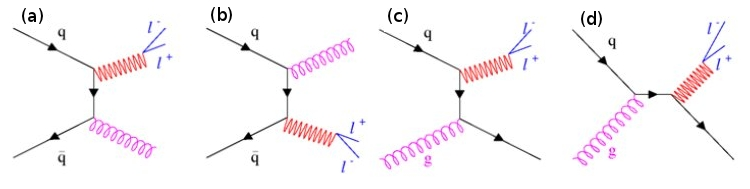
\includegraphics[width=\textwidth]{figures/background/DY.jpeg}
	\caption{The Drell-Yan process has a large range of higher-order QCD corrections that need to be accounted for. 
		(a) and (b) are high order $q\bar{q}$ annihilations, and (c) and (d) are gluon ``Compton scattering'' terms.}
	\label{fig:nlo-dy}
\end{figure}

\section{Drell-Yan and Sea Quark Phenomenology}

\red{Shorten dbar/ubar section? Add pion cloud here? Ref to JC review paper for models.}

\subsection{$\bar{d}/\bar{u}$ Asymmetry}

Even though the quark sea flavor asymmetry is not the main focus of this paper, it is the flagship measurement of the SeaQuest experiment. As such, much of the work that will be explained in later chapters is common to the $\dbar/\ubar$ analysis, and so it is worth touching on its importance here.

The Gottfried Sum Rule (Eq.~\ref{eq:gsr}) can be seen as a measure of flavor symmetry (or asymmetry) in the nucleon. If flavor symmetry were to be upheld, then the sum would strictly be $S_G = \frac{1}{3}$. The New Muon Collaboration (NMC) at CERN sought to test this by measuring the cross section ratio for DIS of muons on hydrogen to muons on deuterium\cite{Amaudruz:1991nw,Arneodo:1994sh}. This cross section ratio allowed for the measurement of $F_2^n/F_2^p$ over a Bjorken-$x$ range of $0.004 < x < 0.8$.  Incident muon energies of \unit[90]{Gev} and \unit[280]{GeV} were used to measure the $F_2$ ratio at $Q^2$ of \unit[4]{GeV$^2$}. The full results of the NMC experiment can be seen to be in clear disagreement with flavor symmetry in Figure~\ref{fig:nmc}. The extrapolated result of the NMC measurements over all $x$ yielded
\begin{equation}
S_G = \int_0^1 dx \left[ \frac{F_2^p - F_2^n}{x} \right] = 0.235 \pm 0.026.
\end{equation}

\begin{figure}[h]
	\centering
	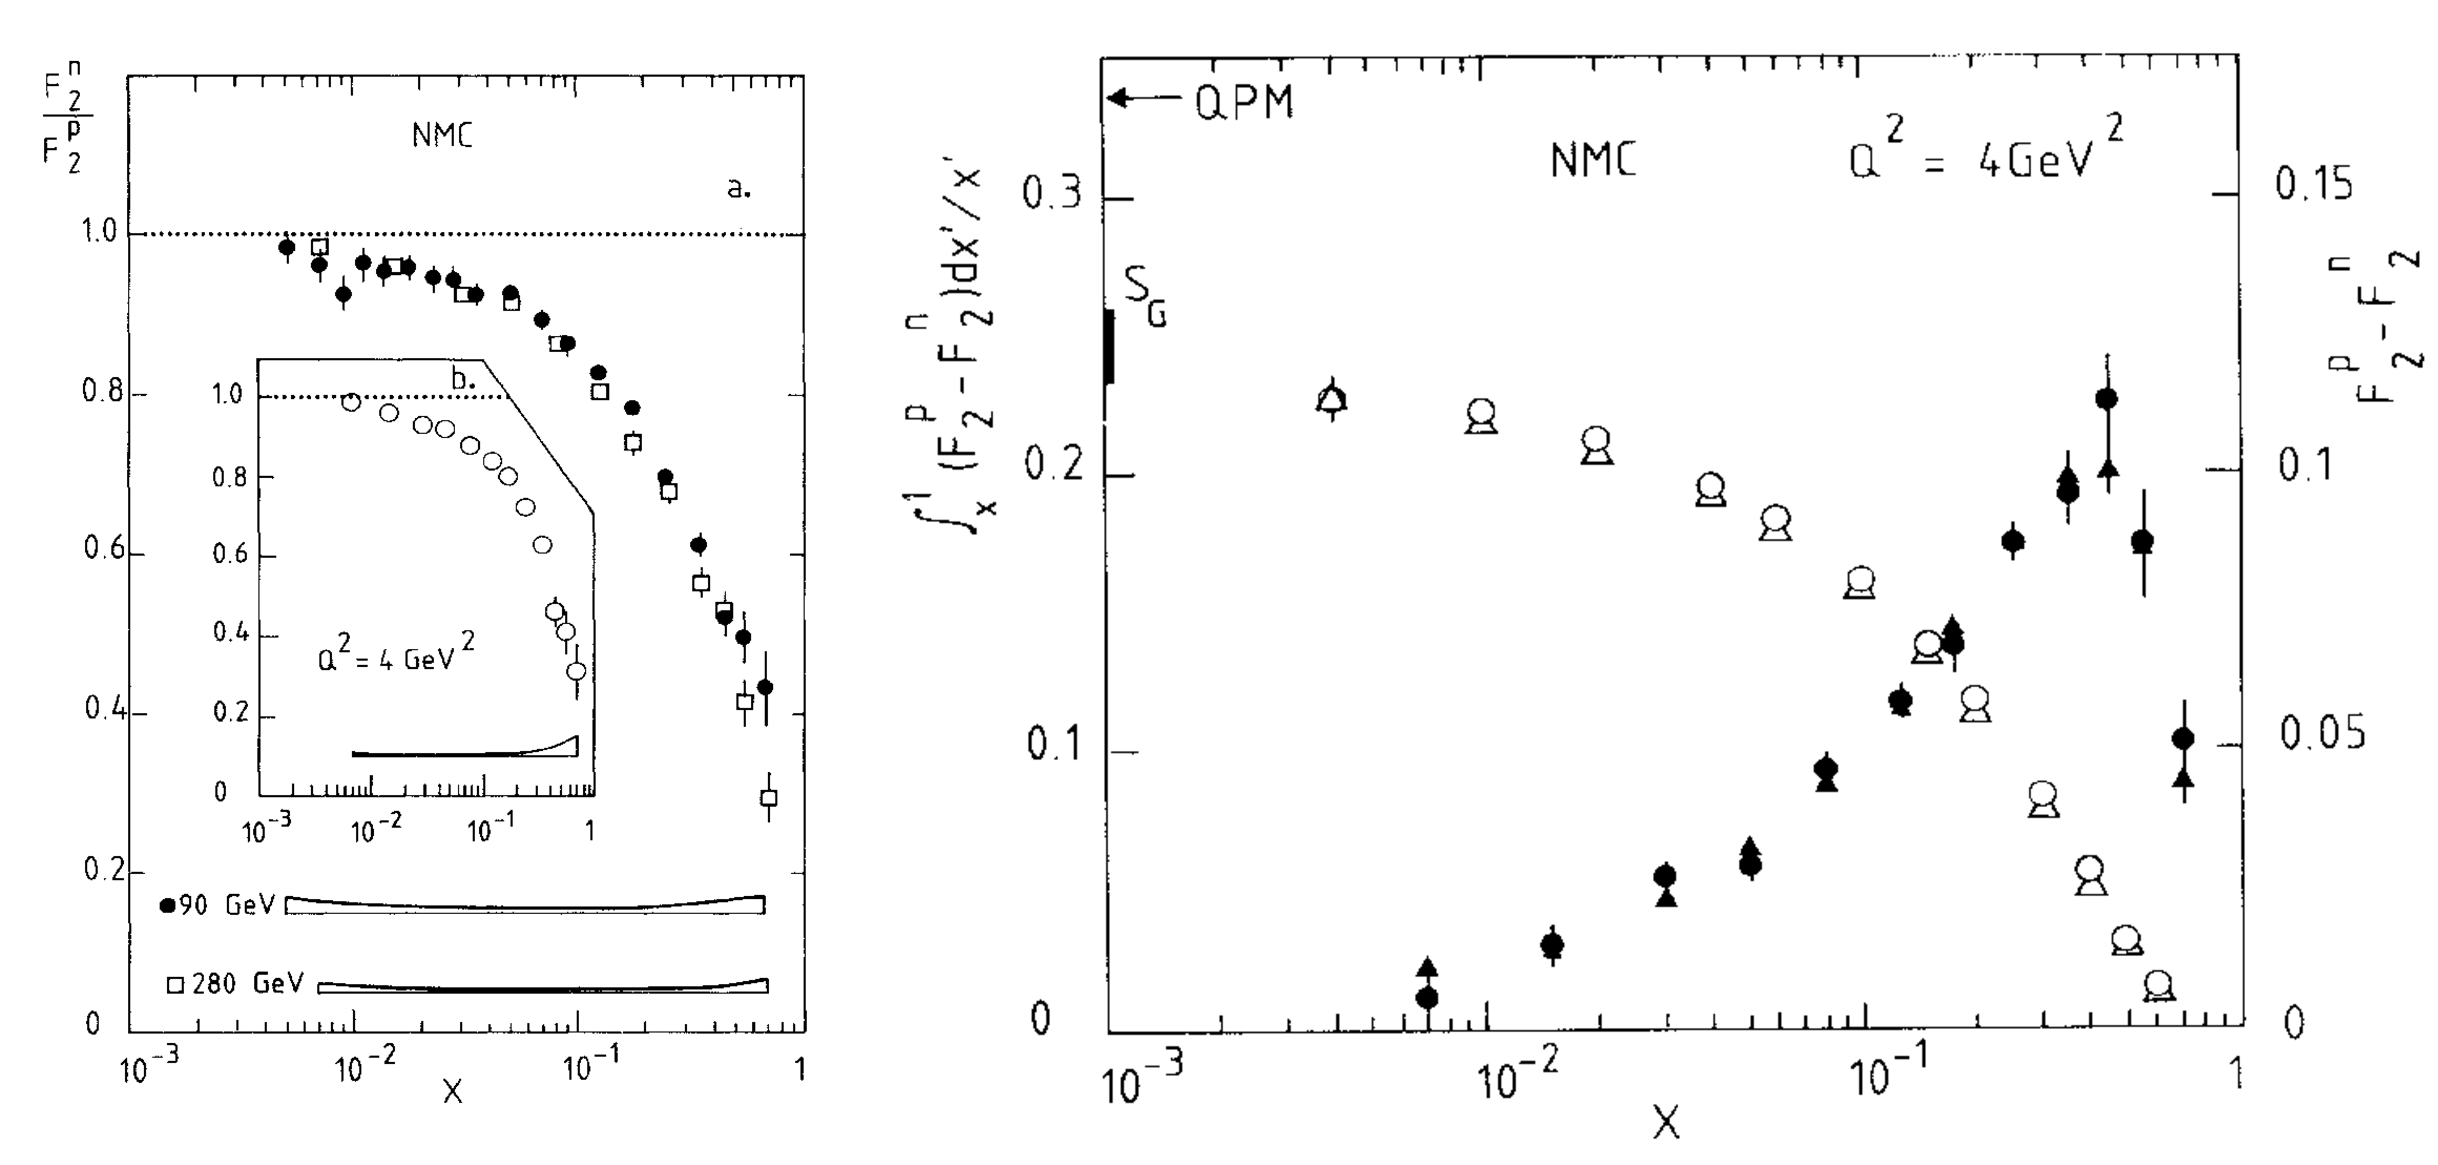
\includegraphics[width=\textwidth]{figures/background/NMC-All.pdf}
	\caption{The NMC experimental measurements of (left) $F_2^n/F_2^p$ and (right) the Gottfried Sum ($S_G$) with $\frac{1}{3}$ denoted by ``QPM''.}
	\label{fig:nmc}
\end{figure}

To reconcile this result with the QPM expectation, certain assumptions need to be reevaluated. The first assumption is that the extrapolation of the NMC result to low $x$ is correct. The second is that charge symmetry is valid. The final assumption is the flavor symmetry of the quark sea, or, $\int dx [\bar{d}(x)] = \int dx [\bar{u}(x)]$. The E-665 experiment at FNAL sought to extend the NMC low-$x$ coverage ($10^-6 < x < 0.3$) despite the difficulties of DIS in the extremely low-$x$ range. The results were consistent with NMC's extrapolation\CN, and so the faulty assumption must lie elsewhere. Charge symmetry violation would lead to such a discrepancy, but to date, charge symmetry has been upheld in the relevant energy regime\cite{Abegg:1998sg}. This leaves only $\int dx [\bar{d}(x)] = \int dx [\bar{u}(x)]$ being violated to account for the difference, and if it were to be the root cause, the contribution to the violation would be
\begin{equation}
\int_0^1 dx[\bar{d}(x) - \bar{u}(x)] = 0.148 \pm 0.039.
\end{equation}
As such, this conclusion was the first indicator pointing to an the existence of more anti-down than anti-up quarks in the quark sea. This prompted further investigation of nucleon sea anti-quark asymmetry.

Following the NMC results, it was suggested\CN to exploit features of the Drell-Yan process as a direct probe of nucleon sea distributions. The most direct method of doing so is to measure the Drell-Yan cross-sections for both hydrogen and deuterium and take the ratio of the two. The proton-deuterium cross section can be seen as a convolution of cross sections of proton-proton and a proton-neutron
\begin{equation}
\sigma^{pd} \approx \sigma^{pp} + \sigma^{pn}
\end{equation}
ignoring any small nuclear effects or phenomenon that may exist in the deuteron. In this picture, the deuterium-to-hydrogen DY ratio yields can be used to determine $\dbar/\ubar$.

The NA51 experiment at CERN\cite{Baldit:1994jk} used a \unit[450]{GeV/c} primary proton beam ($\sqrt{s}=$\unit[29]{GeV}) from CERN-SPS on deuterium and hydrogen targets to measure $\sim$6000 Drell-Yan dimuon events, cutting on $M_{\gamma^*}>$\unit[4.3]{GeV}. The reason for the mass cut is to investigate the Drell-Yan continuum as depicted in Figure~\ref{fig:DY-spectrum} and exclude any possible signal contamination from heavy quarkonia. The NA51 experiment looked to measure what it called the ``p$-$n cross section asymmetry'' of the Drell-Yan process:
\begin{eqnarray}
A_{DY} & = & \frac{\sigma_{pd}-\sigma_{pp}}{\sigma_{pd}+\sigma_{pp}} \\
& = & 2\frac{\sigma_{pp}}{\sigma_{pd}} - 1 \\
A_{DY} & = &  -0.09 \pm 0.02 (\text{stat}) \pm 0.025 (\text{sys})
\end{eqnarray}
which was used to obtain a value for $\dbar/\ubar$. However, due to the NA51 spectrometer being designed to select rapidity about $y=0$ along with having low statistics, NA51 only provided a single value for this measurement centered at $x_F=0$ and $x=0.18$.
\begin{equation}
	\frac{\dbar}{\ubar} \Bigr|_{\langle x \rangle = 0.18} = 1.96 \pm 0.15\text{(stat)} \pm 0.19\text{(sys)}
\end{equation}
This provided strong evidence in confirmation that there was indeed a $\dbar$ excess in the nucleon. Unfortunately, without more statistics, no $x$-dependent behavior of this asymmetry could be determined. This NA51 result coupled with that of NMC prompted several groups to perform global fits from DIS and DY data with the consideration that $\dbar\neq\ubar$, though no $x$-dependent constraints could be imposed on the $\dbar(x)/\ubar(x)$.

An improved experimental design of a ``forward'' muon spectrometer ($x_F>0$) was devised and implemented by the E-866/NuSea experiment to make a more effective measurement of $\dbar/\ubar$. In this kinematic phase space, one can factor in what we know about the PDFs and the DY cross section to consider the measurement as being dominated by the beam quark annihilating with the target's sea anti-quark. If we consider only the regime of $x_1 \gg x_2$,
\begin{eqnarray}
\sigma^{pp} & \propto & \frac{4}{9} u(x_1)\bar{u}(x_2) + \frac{1}{9}d(x_1)\bar{d}(x_2) \\
\sigma^{pn} & \propto & \frac{4}{9} u(x_1)\bar{d}(x_2) + \frac{1}{9}d(x_1)\bar{u}(x_2) \\
\frac{\sigma^{pd}}{2\sigma^{pp}} & \approx & \frac{1}{2} \frac{\left[1 + \frac{1}{4} \frac{d(x_1)}{u(x_1)}\right]}{\left[1 + \frac{1}{4} \frac{d(x_1)}{u(x_1)}\frac{\bar{d}(x_2)}{\bar{u}(x_2)}\right]} \left[1 + \frac{\bar{d}(x_2)}{\bar{u}(x_2)}\right]
\end{eqnarray}
One can approximate even further that since $d(x) \ll 4 u(x)$, then the relation simplifies to
\begin{equation}
\frac{\sigma^{pd}}{2\sigma^{pp}}\Bigr|_{x_1\gg x_2} \approx
\frac{1}{2} \left[1 + \frac{\bar{d}(x_2)}{\bar{u}(x_2)}\right]
\label{eq:866-dbar-ubar}
\end{equation}

The results of the E-866/NuSea measurement\cite{PhysRevLett.80.3715}, along with the NA51 data, can be seen on Figure~\ref{fig:dbar-ubar}. A clear $x$-dependence can be seen as the $\dbar/\ubar$ ratio significantly exceeds unity up to $x_2=0.25$, after which the ratio drops below unity, though not at the same statistical significance. This complex $x$-dependent behavior was not expected by global fits, and many models have been proposed to address it: meson-cloud model, chiral-quark model, Pauli-blocking model, instanton model, chiral-quark soliton model, and more. These are not discussed here, but an in-depth look into each of these can be found in some review articled\cite{Kumano:1997cy, Garvey:2001yq}.

\begin{figure}
	\centering
	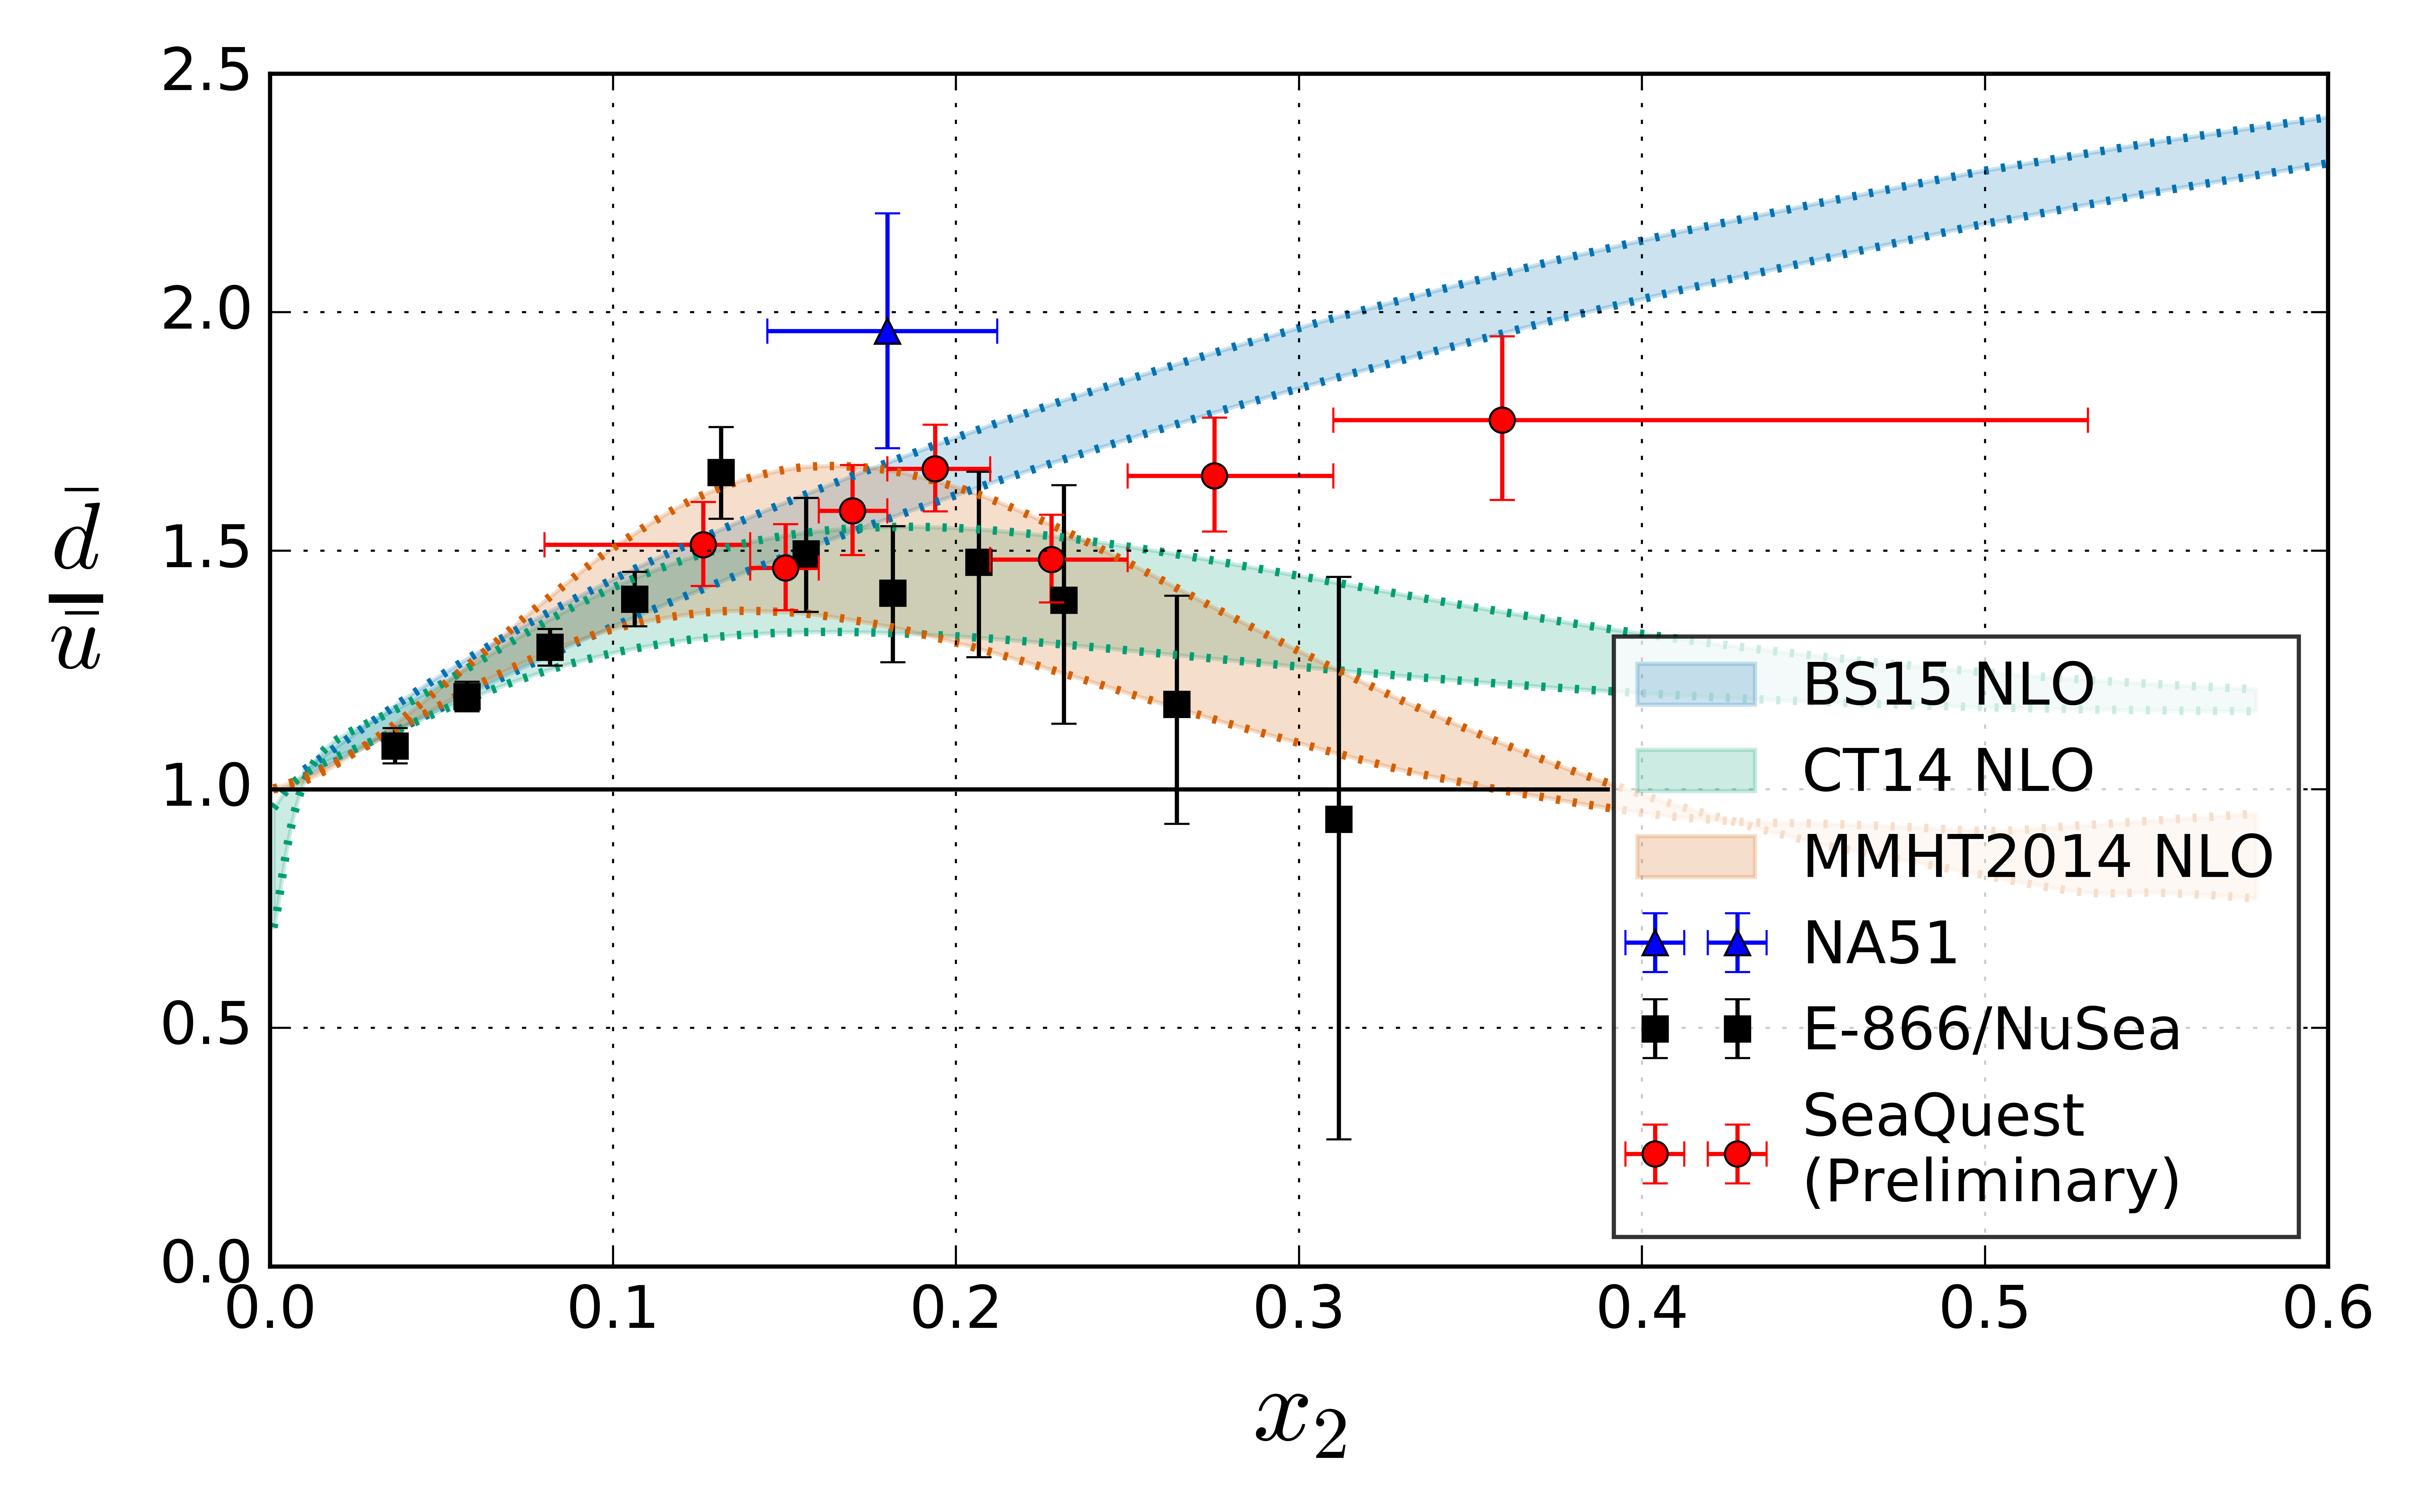
\includegraphics[width=0.75\textwidth]{figures/background/dbar_ubar.png}
	\caption{The measurements and models for the $\dbar/\ubar$ measurement, including the NA51\cite{Baldit:1994jk}, E-866/NuSea\cite{PhysRevLett.80.3715}, and (preliminary) SeaQuest\CN experiments, along with the BS15, CT14, and MMHT models.}
	\label{fig:dbar-ubar}
\end{figure}

In order to study $\dbar(x)/\ubar(x)$ at larger $x$ the SeaQuest collaboration at Fermilab is designed to make precise measurements of proton-induced Drell-Yan cross sections on hydrogen and deuterium targets using the Fermilab Main Injector as a proton source. The relatively lower beam momentum of the Main Injector (\unit[120]{GeV}) provides an opportunity to study parton distributions at larger $x$. This is due to the fact that, as seen in Eq.~\ref{eq:DY-cross}, for fixed x, the Drell-Yan cross section is inversely proportional to the square of the center-of-mass energy, $s$. Another benefit of utilizing a lower-energy beam is that the primary background, $\Jpsi$ production, which limited the instantaneous luminosity in E-866/NuSea, scales with s, and is thereby reduced, allowing the usage of a more intense proton beam.

Given these factors above and anticipated run time of the SeaQuest experiment, the range of $0.1<x_2<0.45$ is expected to be covered. In the run time since commissioning in 2012, enough data has been analyzed to yield a preliminary $\dbar(x)/\ubar(x)$ result, which can be seen in Figure~\ref{fig:dbar-ubar}. This measurement and its analysis is being led by Bryan Kerns from the University of Illinois at Urbana-Champaign. Further details regarding this topic can be found in his dissertation and forthcoming publication(s).

\subsection{Pion Cloud Model}

\red{???}

\section{The Nuclear EMC Effect}

\red{Mention pT wherever it comes up!}

Approximately ten years before the NMC experiment's discovery of the $\dbar(x)\neq\ubar(x)$ discovery, the European Muon Collaboration (EMC) at CERN, in 1983, measured the ratios of the structure functions of iron and deuterium over a large kinematic range using the DIS of muons\cite{Aubert:1983xm}. The result has been repeatedly scrutinized, studied, and confirmed. It was discovered that the structure function of a nucleon bound in a nucleus is fundamentally modified from that of a free nucleon. The nucleus was na\:{i}vely understood as a simple convolution of many nucleons, and that the partonic structure functions of bound and free nucleons should be identical. This assumption was found to not hold against actual measurements, and the observed behavior holds true across all heavy nuclei. This effect can be interpreted as a \emph{modification of quark and gluon distributions in bound nucleons by the nuclear environment}. In this section, the history and collective behavior known as ``The EMC Effect'' will be reviewed, a quantitative A-dependent measure of the effect will be defined, and models that attempt to explain the phenomenon will be discussed. Lastly, the contributions of SeaQuest and previous Drell-Yan experiments to the study of the EMC Effect will be explored.

\subsection{Historical Overview} \label{ssec:emc-history}

\begin{figure}
	\centering
	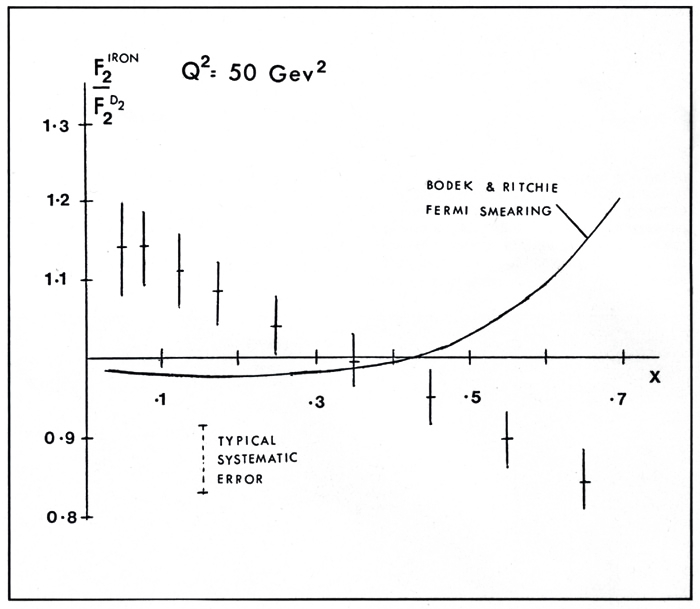
\includegraphics[height=0.35\textheight]{figures/background/emc_effect_original-v2.jpg}
	\caption{The original EMC ratio measurement by the EMC collaboration\cite{Aubert:1983xm}. Overlaid is the na\:{i}ve, expected ratio taking into account only the Fermi motion of the nucleons in the heavy nucleus.}
	\label{fig:emc-one-naive}
\end{figure}

Unpolarized inclusive lepton scattering is a process that uses an energized lepton to investigate nucleon structure, and it specifically depends on two independent variables: $Q^2$ and Bjorken-$x$ (sometimes referred to as $x_B$, but here left as $x$).
\begin{equation}
	Q^2 = -q^2\ \ ;\ \ x = \frac{Q^2}{2 m_p \omega}
\end{equation}
where $q$ is the transferred four-momentum, $x_B$ is the same Bjorken-x scaling variable as is in the PDF section mentioned above, $m_p$ is the proton mass, and $\omega$ is the transferred energy in the proton rest frame. At energies of $Q^2>$\unit[2]{(GeV/c)$^2$}, the parton substructure is revealed and the inelastic structure function, $F_2$ is able to be measured. The EMC group extracted the ratio $F_2^{Fe}(x,Q^2)/F_2^{d}(x,Q^2)$, where these are the average bound nucleon structure functions in iron and deuterium. This was done by measuring the DIS \emph{per nucleon cross section ratio}, which can be expressed as\cite{Halzen:1984mc}:
\begin{equation}
\frac{\sigma^{A_1}/A_1}{\sigma^{A_2}/A_2} = \frac{F_2^{A_1}(x, Q^2)}{F_2^{A_2}(x, Q^2)} \cdot \frac{\left[ 1 + 2\frac{1+\omega^2/Q^2}{R_{A_1}-1}\tan^2\frac{\theta}{2} \right]}{\left[ 1 + 2\frac{1+\omega^2/Q^2}{R_{A_2}-1}\tan^2\frac{\theta}{2} \right]} \approx \frac{F_2^{A_1}(x, Q^2)}{F_2^{A_2}(x, Q^2)}
\end{equation}
where $\theta$ is the lepton scattering angle and $R_A=\sigma^A_L/\sigma^A_T$ is the ratio of the longitudinal to transverse cross section for nucleus A. The A-dependence of $R_A$ will be discussed later, but for now, let us assume that $R$ does not exhibit a nuclear dependence, and the per nucleon cross section ratio therefore approximates nicely to the ratio of the structure functions. For $0.4\gtrsim x\lesssim0.6$ where nucleon Fermi motion effects can be neglected, the expectation was to measure unity, which would indicate that the structure function of a deeply bound nucleon and loosely bound nucleons are identical. With this goal in mind, they chose $^{56}Fe$ and deuterium, as iron is the most tightly bound nucleus at $E^{Fe}_{\text{bind}}=$\unit[8.8]{MeV/nucleon} and deuterium is as close to being a free nucleon as possible while still being a symmetric nuclei ($N=Z=A/2$) with a binding energy of only $E^{d}_{\text{bind}}=$\unit[2.2]{MeV/nucleon}. The reason to perform this experiment is that, if this mearuement showed unity in the regions not affected by Fermi motion, then heavy nuclei could be used to gain a luminosity boost when studying the free nucleon structure functions. Instead, they observed the measured cross-section ration being 1 at $x\approx 0.3$ and then steadily declining to a value of about 0.8 at $x\approx0.7$ (Figure~\ref{fig:emc-one-naive})	
	
At the time of the measurement was presented, the result astounded the physics community. They could hardly believe that high momentum transfers that were many times larger than the nuclear binding energies that the quark distributions should be altered by the nuclear mean field. This result was confirmed only three months later by the SLAC-MIT-Rochester group that re-examined its data for DIS on steel\cite{PhysRevLett.50.1431} and found the same behavior, as can be seen in Figure~\ref{fig:emc-e87}. This opened the gates to an enormous amount of activity in both experiment and theory to fully characterize the phenomenon, resulting at present more than 1100 citations of the original EMC publication\cite{Aubert:1983xm}. \setlength{\columnsep}{28pt} \begin{wrapfigure}{r}{0pt}
	\centering
	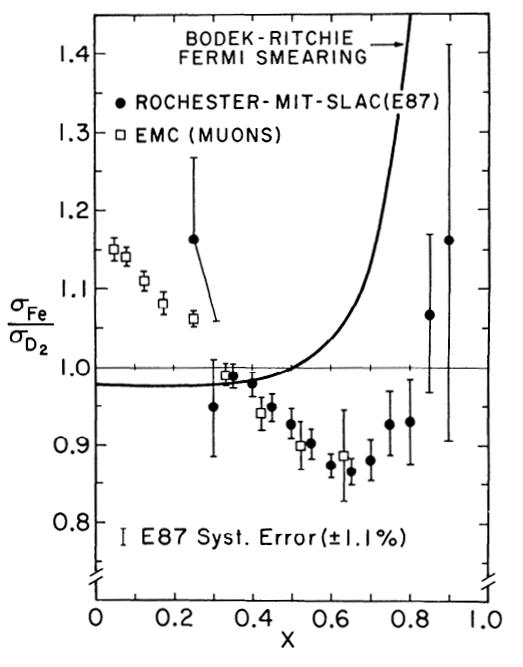
\includegraphics[height=0.35\textheight]{figures/background/SLAC-E87.png}
	\caption{SLAC E-87 was quick to report its own finding months later confirming EMC's observation\cite{PhysRevLett.50.1431}.}
	\vspace{-20pt}
	\label{fig:emc-e87}
\end{wrapfigure} The compendium of experimental data and theory papers have been discussed in great detail in the excellent review papers by Geesaman~\cite{Geesaman:1995yd} in 1995 and Norton~\cite{norton:emc-review} in 2003. As such, I will only summarize the main theoretical ideas and the most prominent interpretation of the effect. A visual summary of EMC data can be found in Figure~\ref{fig:emc-all-targ} where data from EMC~\cite{Aubert:1983xm}, SLAC~\cite{Arnold:1983mw, Gomez:1993ri}, BCDMS~\cite{Benvenuti:1987az}, NMC~\cite{Amaudruz:1991nw}, and HERMES~\cite{Ackerstaff:1999ac} is plotted for nine different targets.

\begin{figure}
	\centering
	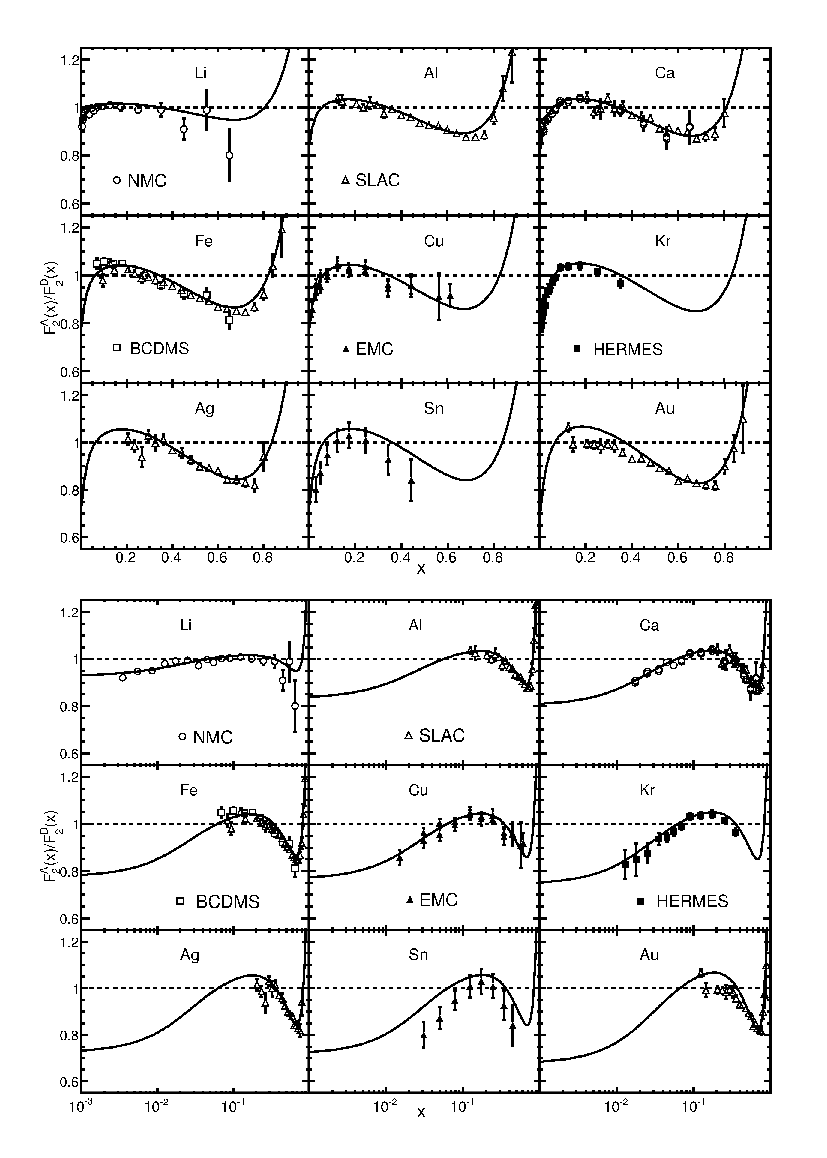
\includegraphics[height=0.9\textheight]{figures/background/emc-all-targ.eps}
	\caption{A compilation of data regarding the measurement of $F^A_2/F_2^D$ for nine different heavy targets with an overlaid fit by Chen et al.\cite{Chen:2013oga}.}
	\label{fig:emc-all-targ}
\end{figure}

\subsection{\texorpdfstring{Universal $x$-dependence}{Universal x-dependence}}

The SLAC E139 experiment provides very precise information for the high-$x$ range ($x>0.2$) for many nuclei. The high-energy electron DIS data from SLAC E61~\cite{Stein:1975yy} and HERMES~\cite{Ackerstaff:1999ac} experiments along with the muon DIS data from NMC~\cite{Amaudruz:1991nw} supplements this with the very low-$x$ range. Finally, the more recent data from JLAB-E03103~\cite{Seely:2009gt} that uses a relatively low energy beam (\unit[5.8]{GeV}) provides data for the high-$x$ Fermi motion area ($0.85<x<0.95$). These together help to paint a full characteristic picture of the $x-$dependence of this $\sigma^A/\sigma^d$ ratio, which has been found to be universal for all $A>2$. A visualization of some of this data for carbon and nitrogen  the measurement up into four qualitative regions of this ratio can be seen in Figure~\ref{fig:emc-regions}.
\begin{figure}
	\centering
	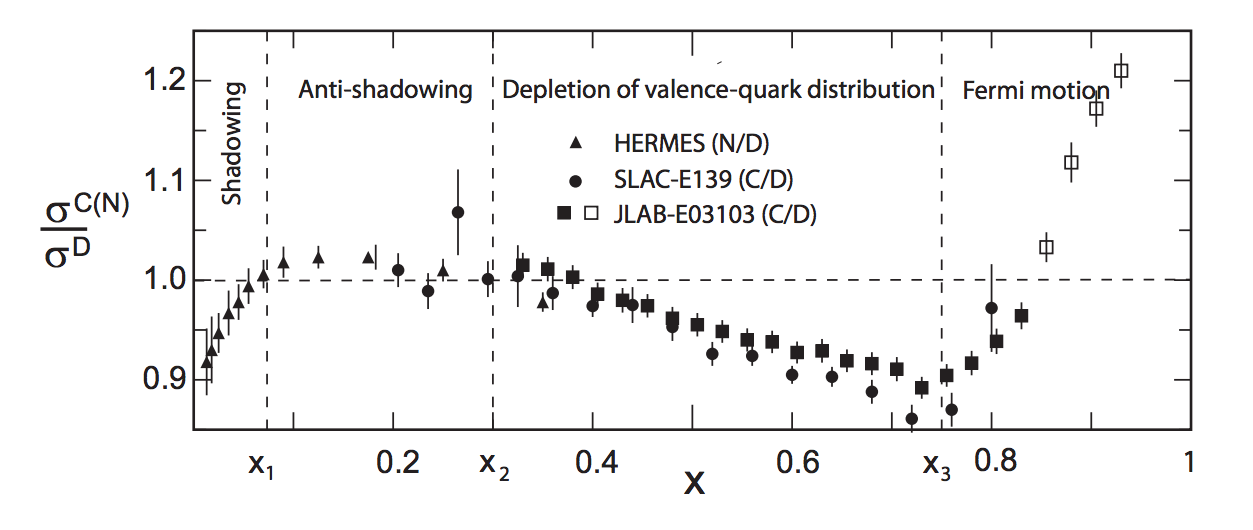
\includegraphics[width=\textwidth]{figures/background/emc-regions.png}
	\caption{The ratio of $\sigma^{C(N)}/\sigma^d$ covering nearly the entire $x\in[0,1]$ interval~\cite{Rith:2014tma}. The four qualitative regions are denoted by roughly chosen boundaries $x_1, x_2, x_3$ (not to be confused with the beam and target $x_1$ and $x_2$ used in the rest of this paper).}
	\label{fig:emc-regions}
\end{figure}
\begin{itemize}
	\item $\mathbf{0<x\lesssim0.06:}$ The ``shadowing'' region where the ratio is less than unity and decreasing as $x\rightarrow0$. The dominant contribution to the cross section in this kinematic regime is from sea quarks.
	\item $\mathbf{0.06\lesssim x \lesssim 0.3:}$ The (perhaps poorly named) ``anti-shadowing'' region exhibits a very slight rise of the ratio above unity. In general, this range of values represent only a transition region between its two bookending effects.
	\item $\mathbf{0.3\lesssim x \lesssim 0.8:}$ The ratio becomes significantly smaller than unity, decreasing with increasing $x$. This is of key focus for this paper, and this region is what is generally referred to as the \emph{``EMC Effect''}\cite{Geesaman:1995yd} as it is the only part of the phenomenon that is not fully understood.  As far as DIS goes, the sea quark contribution is essentially negligible, given the current understanding of quark PDF's, and the behavior is dominated by valence quark distributions.
	\item $\mathbf{0.8\lesssim x < 1:}$ The ratio increases rapidly with increasing $x$. This is dominated by a kinematic effect of the free nucleon cross section vanishing as $x\rightarrow1$. It is also due to the effect of Fermi motion of the bound nucleons in the nucleus.
\end{itemize}

\subsection{Nuclear Dependence of R}

It was stated in section~\ref{ssec:emc-history} that the per nucleon cross section ratio only reduces to the ratio of structure functions in the case that $R=\sigma_L/\sigma_T$ is A-independent. This particular measurement was the focus of experiments SLAC-E140~\cite{PhysRevLett.61.1061, Dasu:1993vk}, NMC~\cite{Arneodo:1996qe}, and HERMES~\cite{Ackerstaff:1999ac}. A re-analysis of all SLAC data with improved corrections~\cite{Dasu:1993vk} showed that the difference in $R$ between iron and deuterium is consistent with zero ($R_{Fe}-R_d = 0.001 \pm 0.018 (\text{stat}) \pm 0.016 (\text{sys.})$), and that there are no significantly different spin-0 constituents or higher twist effects in nuclei as compared to free nucleons. Later on, results from HERMES corroborated these findings. The ratio of $R_A/R_d$ were derived from the NMC and SLAC results for $\Delta R = R_A - R_d$ and reported an averaged value of $R_A/R_d = 0.99 \pm 0.03$, providing further agreement on the A-independence of $R$.

A recent study by Guzey et al.~\cite{Guzey:2012yk} looked to data from SLAC E139, BCDMS, and EMC to examine the impact of $R$ on the extraction of $F_2^A/F_2^d$ and $F_1^A/F_1^d$ from $\sigma^A/\sigma^d$ data. They demonstrate the presence of a small but non-zero difference between $R$ for nuclei and free nucleons. While this does appear to effect the extraction of the nuclear enhancement in the ratio of the $F_1^A/F_1^d$, the extraction of $F_2^A/F_2^d$ appears to remain unaffected. As such, this thesis assumes that it is safe to assume that $\sigma^A/\sigma^d \approx F_2^A/F_2^d$.

\subsection{$Q^2$ Dependence of EMC Effect}

\begin{figure}[!b]
	\centering
	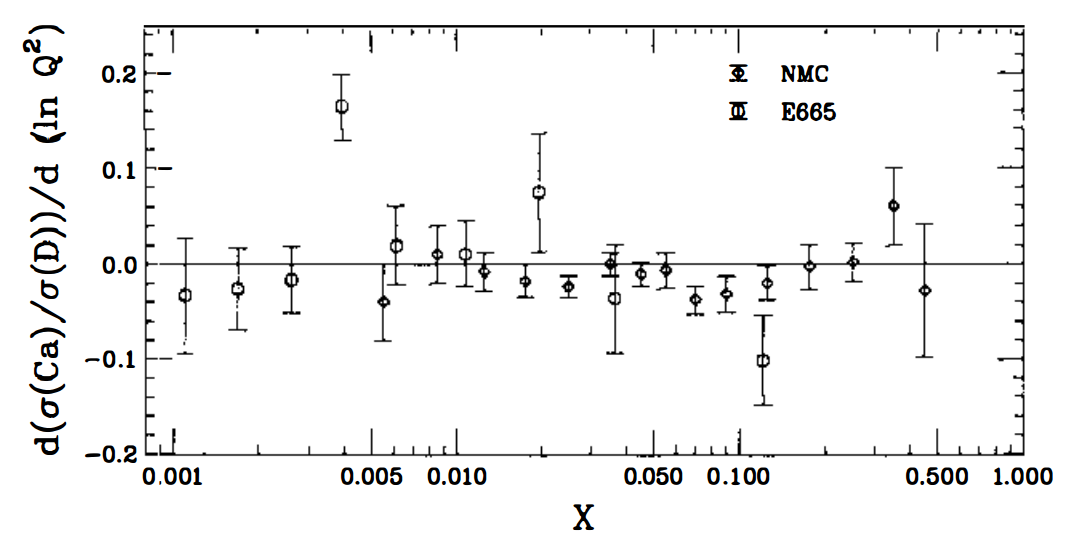
\includegraphics[width=0.8\textwidth]{figures/background/emc-q2-dep.png}
	\parbox{4.5in}{\caption{Measurements of the change in the $\sigma^{Ca}/\sigma^d$ ratio with respect to $\ln Q^2$  over a broad range of $x$~\cite{Geesaman:1995yd}.}
	\label{fig:emc-q2-dep}}
\end{figure}
It is important when investigating structure functions and quark/gluon distributions to pay attention to the $Q^2$ sensitivity of the measurements. Nuclear structure functions can be directly interpreted as parton distributions only if $Q^2$ is large enough to precisely define the light-cone direction and reduce higher-twist contributions. The first condition places a restriction on $x^2/Q^2$ and is usually well satisfied, even at relatively low values of $x$ and $Q^2$. However, the value of the higher-twist terms is under little theoretical control, and these terms can have specific nuclear dependences. 

Experimentally, the verdict was very clear from the agreement of muon and electron DIS data that any $Q^2$ dependence must be very small since, at the same value of $x$, their average $Q^2$ differs by more than an order of magnitude. The lack of $Q^2$ dependence can be seen in Figure~\ref{fig:emc-q2-dep} which shows the derivative of DIS cross section with respect to $\ln Q^2$ over a broad range of $x$, combining NMC and E665 data for calcium~\cite{Geesaman:1995yd}.  \emph{This absence of any observable dependence of the ratio on $Q^2$ justifies the usual practice of combining all the $Q^2$ data at a fixed $x$-value to display the $x$-dependence of the ratio}. The only measurement that seems to refute this conclusion is a measurement of $\sigma^{Sn}/\sigma^C$ by NMC which observes a statistically significant, yet small $Q^2$ dependence at small values of $x$ ($x\lesssim 0.06$)~\cite{Arneodo:1996qe}. Due to the large amount of evidence to the contrary along with the fact that SeaQuest is only sensitive to $x\gtrsim0.08$, this paper will move forward with the the understanding that there is no $Q^2$ dependence in this ratio measurement. As such, this paper will frequently abbreviate such expressions:
\begin{equation}
\frac{F_2^A(x, Q^2)}{F_2^d(x, Q^2)} \rightarrow \frac{F_2^A(x)}{F_2^d(x)}\ \ \ ;\ \ \ \frac{2}{A}\frac{\sigma^A(x, Q^2)}{\sigma^d(x, Q^2)} \rightarrow \frac{2}{A} \frac{\sigma^A(x)}{\sigma^d(x)}
\end{equation}
when in reality it is only the ratio that is $Q^2$-independent.

\subsection{Shadowing}

Even though the ``shadowing'' region of the EMC effect ($x\lesssim 0.06$) is outside of the kinematic acceptance of the SeaQuest experiment ($x\gtrsim0.08$), it is certainly worth briefly discussing this interpretation. This term ``shadowing'' has been introduced to explain the reduction of the nuclear cross sections in photoproduction, but in this particular case, has also been used in discussing very low-$x$ modifications to the nuclear cross section in DIS. 

The generally accepted explanation for this modification is that the parton distributions in bound nucleons actually \emph{remain unchanged} compared to those in free nucleons. In the rest frame of the \emph{nucleus}, the nuclear effect is attributed to the modification of the interaction of the virtual photon with the atomic nucleus by fluctuations of the virtual photon into quark-antiquark pairs. This pair then interacts with the nucleus via the strong interaction instead of electromagnetically. As a result of this increase in strength, the interaction no longer proceeds incoherently with all the rest of the nucleons, but \emph{preferentially with those at the front surface}. The other nucleons in the ``shadow'' of the nucleons in front are much less likely to interact, and thereby do not (or much less) contribute to the cross section. As a result, when calculating the per nucleon cross section ratio $\frac{\sigma^A/A}{\sigma^d/2}$ and the deuteron essentially has the same cross section as the heavy nucleus (in this specific regard), then the ratio value will be suppressed.  

Quantitatively, this behavior will occur when the $q\bar{q}$ pair fluctuation exists for longer than the mean free path of the pair in a nucleus (distance between nucleons). The fluctuation length behaves as $\Delta d \approx 1/Mx$ where $M$, the effective mass of the $q\bar{q}$ pair is approximately \unit[1.1]{GeV}~\cite{Kopeliovich:2012kw}, yielding a fluctuation distance of $\Delta d \approx \unit[0.2]{fm}/x$. This becomes larger than the mean free path $L\simeq\unit[2.5]{fm}$ when $x\lesssim 0.08$.

\subsection{Fermi Motion}

\begin{wrapfigure}{r}{0pt}
	\centering
	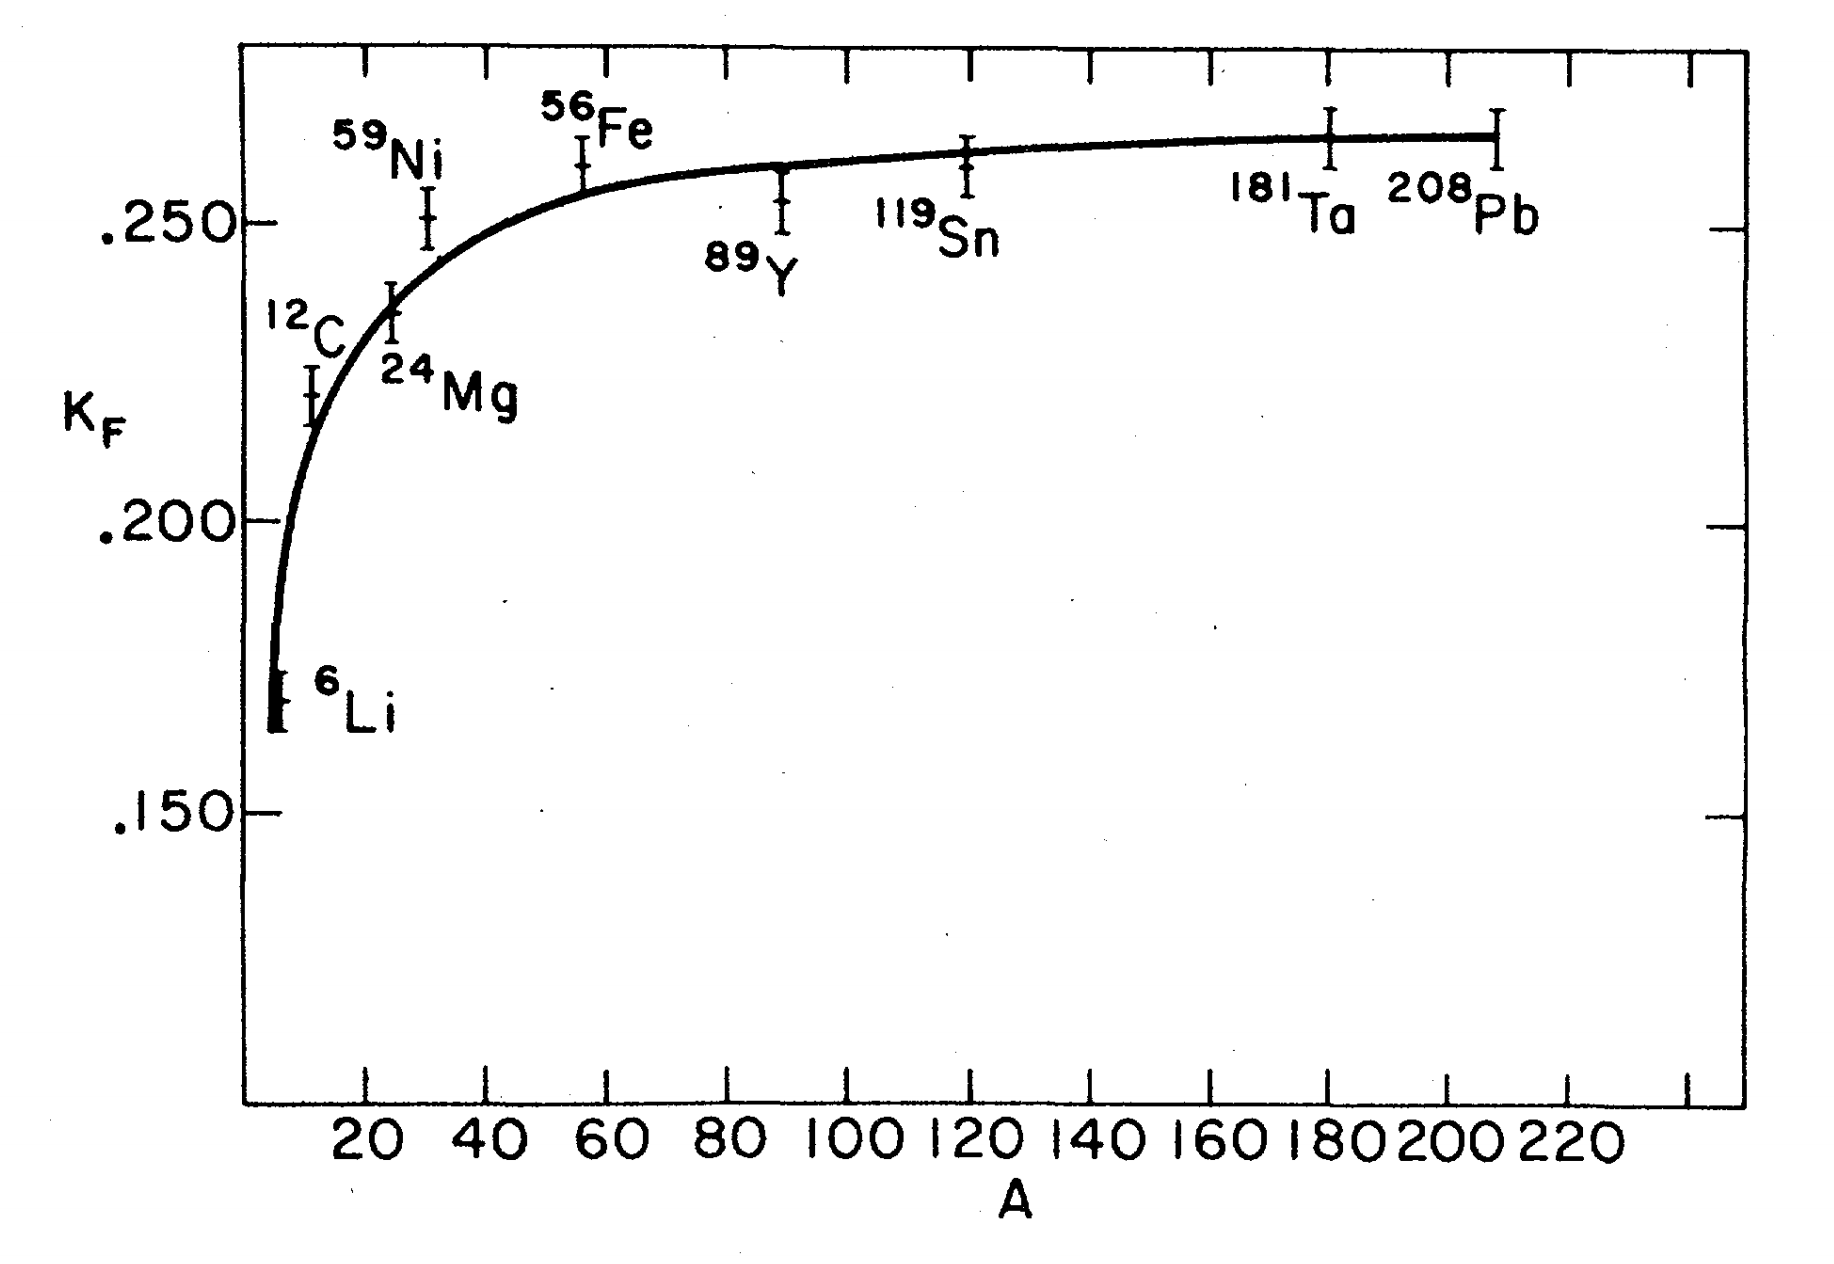
\includegraphics[width=0.45\textwidth]{figures/background/fermi-momentum.png}
	\caption{The Fermi momenta $K_F$ (in GeV) for various nuclei of atomic weight A~\cite{PhysRevD.23.1070}.}
	\vspace{-20pt}
	\label{fig:fermi-momentum}
\end{wrapfigure}
One of the more striking features of the $F_2^A(x)/F_2^d(x)$ is the sharp rise in the ratio value at high-$x$ ($0.8\nobreak\lesssim\nobreak x\nobreak\lesssim\nobreak1$). This feature arises as a result of the quantum mechanical principle of Fermi motion, which arises from the confinement of nucleons within the nucleus. If one considers the uncertainty principle inherent in all wave-like systems, $\sigma_x \sigma_p \geq \frac{\hbar}{2}$, there is a direct effect on the momentum distribution of nucleons when one considers the the spatial localization of bound nucleons in a nucleus. For example, the nucleons in a tightly bound nucleus (like iron) must have a more precise spatial localization (smaller $\sigma_x$) than a nucleon in a more loosely bound nucleus (such as the deuteron). As a result, the magnitute of momentum variations will be greater in the case of iron than in the deuteron (an effect sometimes called ``Fermi smearing''). The magnitude of the Fermi momenta of several nuclei can be found in Figure~\ref{fig:fermi-momentum}.

In the extreme case of a free nucleon (which deuterium is chosen to approximate as best as possible), there exists no Fermi motion, as the nucleon is unbound. As a result, the $F_2$ structure function must vanish as $x\rightarrow1$ as it becomes very unlikely that a single quark will possess a large fraction of the momentum of the free nucleon without the help of quantum mechanical fluctuations and Fermi smearing. In the case of the deuteron though, there is still some Fermi motion, as it still consists of two bound nucleons. Bodek and Ritchie were among the first to lay out a model for comparing this effect and how it would differ between different nuclei~\cite{PhysRevD.23.1070}.  The model of how this would affect the structure function ratio is seen on the original EMC plot in Figure~\ref{fig:emc-one-naive}, given no other nuclear effects (such as the EMC Effect).

As is the case with shadowing, this regime is far beyond the kinematic acceptance of SeaQuest to measure. There is still good reason to believe that, whatever the cause of the EMC effect, it likely overlays the effect of Fermi motion, which, depending on the model, can effect the ratio measurement above $x\approx0.5$. Even with this estimate, there are very few SeaQuest statistics at this $x$-range.

\subsection{A-dependence of EMC Effect Slope}

\begin{table}
	\centering
	\ra{1.2}
	\setlength{\tabcolsep}{2em}
	\begin{tabular}{@{}lllll@{}}\toprule
		Nucleon & & $dR_{EMC}/dx$~\cite{Seely:2009gt} & $dR_{EMC}/dx$~\cite{Gomez:1993ri} & $dR_{EMC}/dx$ (comb.) \\ \midrule	
		$^2H$ & & 									 & 								  & -0.10$\pm$0.05~\cite{Griffioen:2015hxa} \\
		$^3He$ & & -0.070$\pm$0.029 	& 								& -0.070$\pm$0.029 \\
		$^4He$ & & -0.199$\pm$0.029		& -0.191$\pm$0.061   & -0.191$\pm$0.026 \\
		$^9Be$ & & -0.271$\pm$0.029		 & -0.207$\pm$0.037  & -0.243$\pm$0.023 \\
		$^{12}C$ & & -0.280$\pm$0.029	& -0.318$\pm$0.040  & -0.292$\pm$0.023 \\
		$^{27}Al$ & & 								& -0.325$\pm$0.034  & -0.325$\pm$0.034 \\
		$^{40}Ca$ & & 								& -0.350$\pm$0.047 & -0.350$\pm$0.047 \\
		$^{56}Fe$ & & 								& -0.388$\pm$0.032 & -0.388$\pm$0.032 \\
		$^{108}Ag$ & & 								& -0.496$\pm$0.051 & -0.496$\pm$0.051 \\
		$^{197}Au$ & & 								& -0.409$\pm$0.039 & -0.409$\pm$0.039 \\ \bottomrule		
	\end{tabular}
	\caption{Measured EMC slopes $dR_{EMC}/dx$ for $0.35\leq x \leq 0.7$~\cite{Piasetzky:2011zz}.}
	\label{tab:emc-slopes}
\end{table}

Precise measurements of $R_{EMC}=(F_2^A/A)/(F_2^d/2)$ for various nuclei, from $^3He$ to $^{197}Au$ have been analyzed, and the intermediate-to-high $x$ region ($0.35<x<0.7$) shows a declining behavior that can be fit with a line. The slope of this line has become the focus of study when attempting to interpret the EMC effect, as this slope ($dR_{EMC}/dx$) exhibits a significant A-dependence. The magnitudes of the slopes appear to increase with increasing $A$. The table of values of $dR_{EMC}/dx$ for various nuclei can be found in Table~\ref{tab:emc-slopes}.

The intial attempt at understanding this was to interpret it as some effect of nuclear density. Since the effect of nuclear density on a given nucleus is due to the presence of the other ($A-1$) nucleons, the slope $|dR_{EMC}/dx|$ was plotted against the average nuclear density scaled down by a factor of $(A-1)/A$ in order to remove the struck nucleon’s contribution to the average nuclear density. The result for light nuclei was shown by Seely \emph{et al.} to have interesting result, as is seen in Figure~\ref{fig:emc-slope-vs-density}. The most notable result was a definite overall trend with $^9Be$ representing a significant outlier. It has been theorized that $^9Be$ is an outlier due to its nuclear structure resembling two $\alpha-$particles ($^4He$ nuclei) with an extra nuclei. This would mean that perhaps it is not the average nuclear density, but the \emph{local} nuclear density, or density about the struck nucleon. There is still a missing piece needed to represent this density.

\begin{figure}
	\centering
	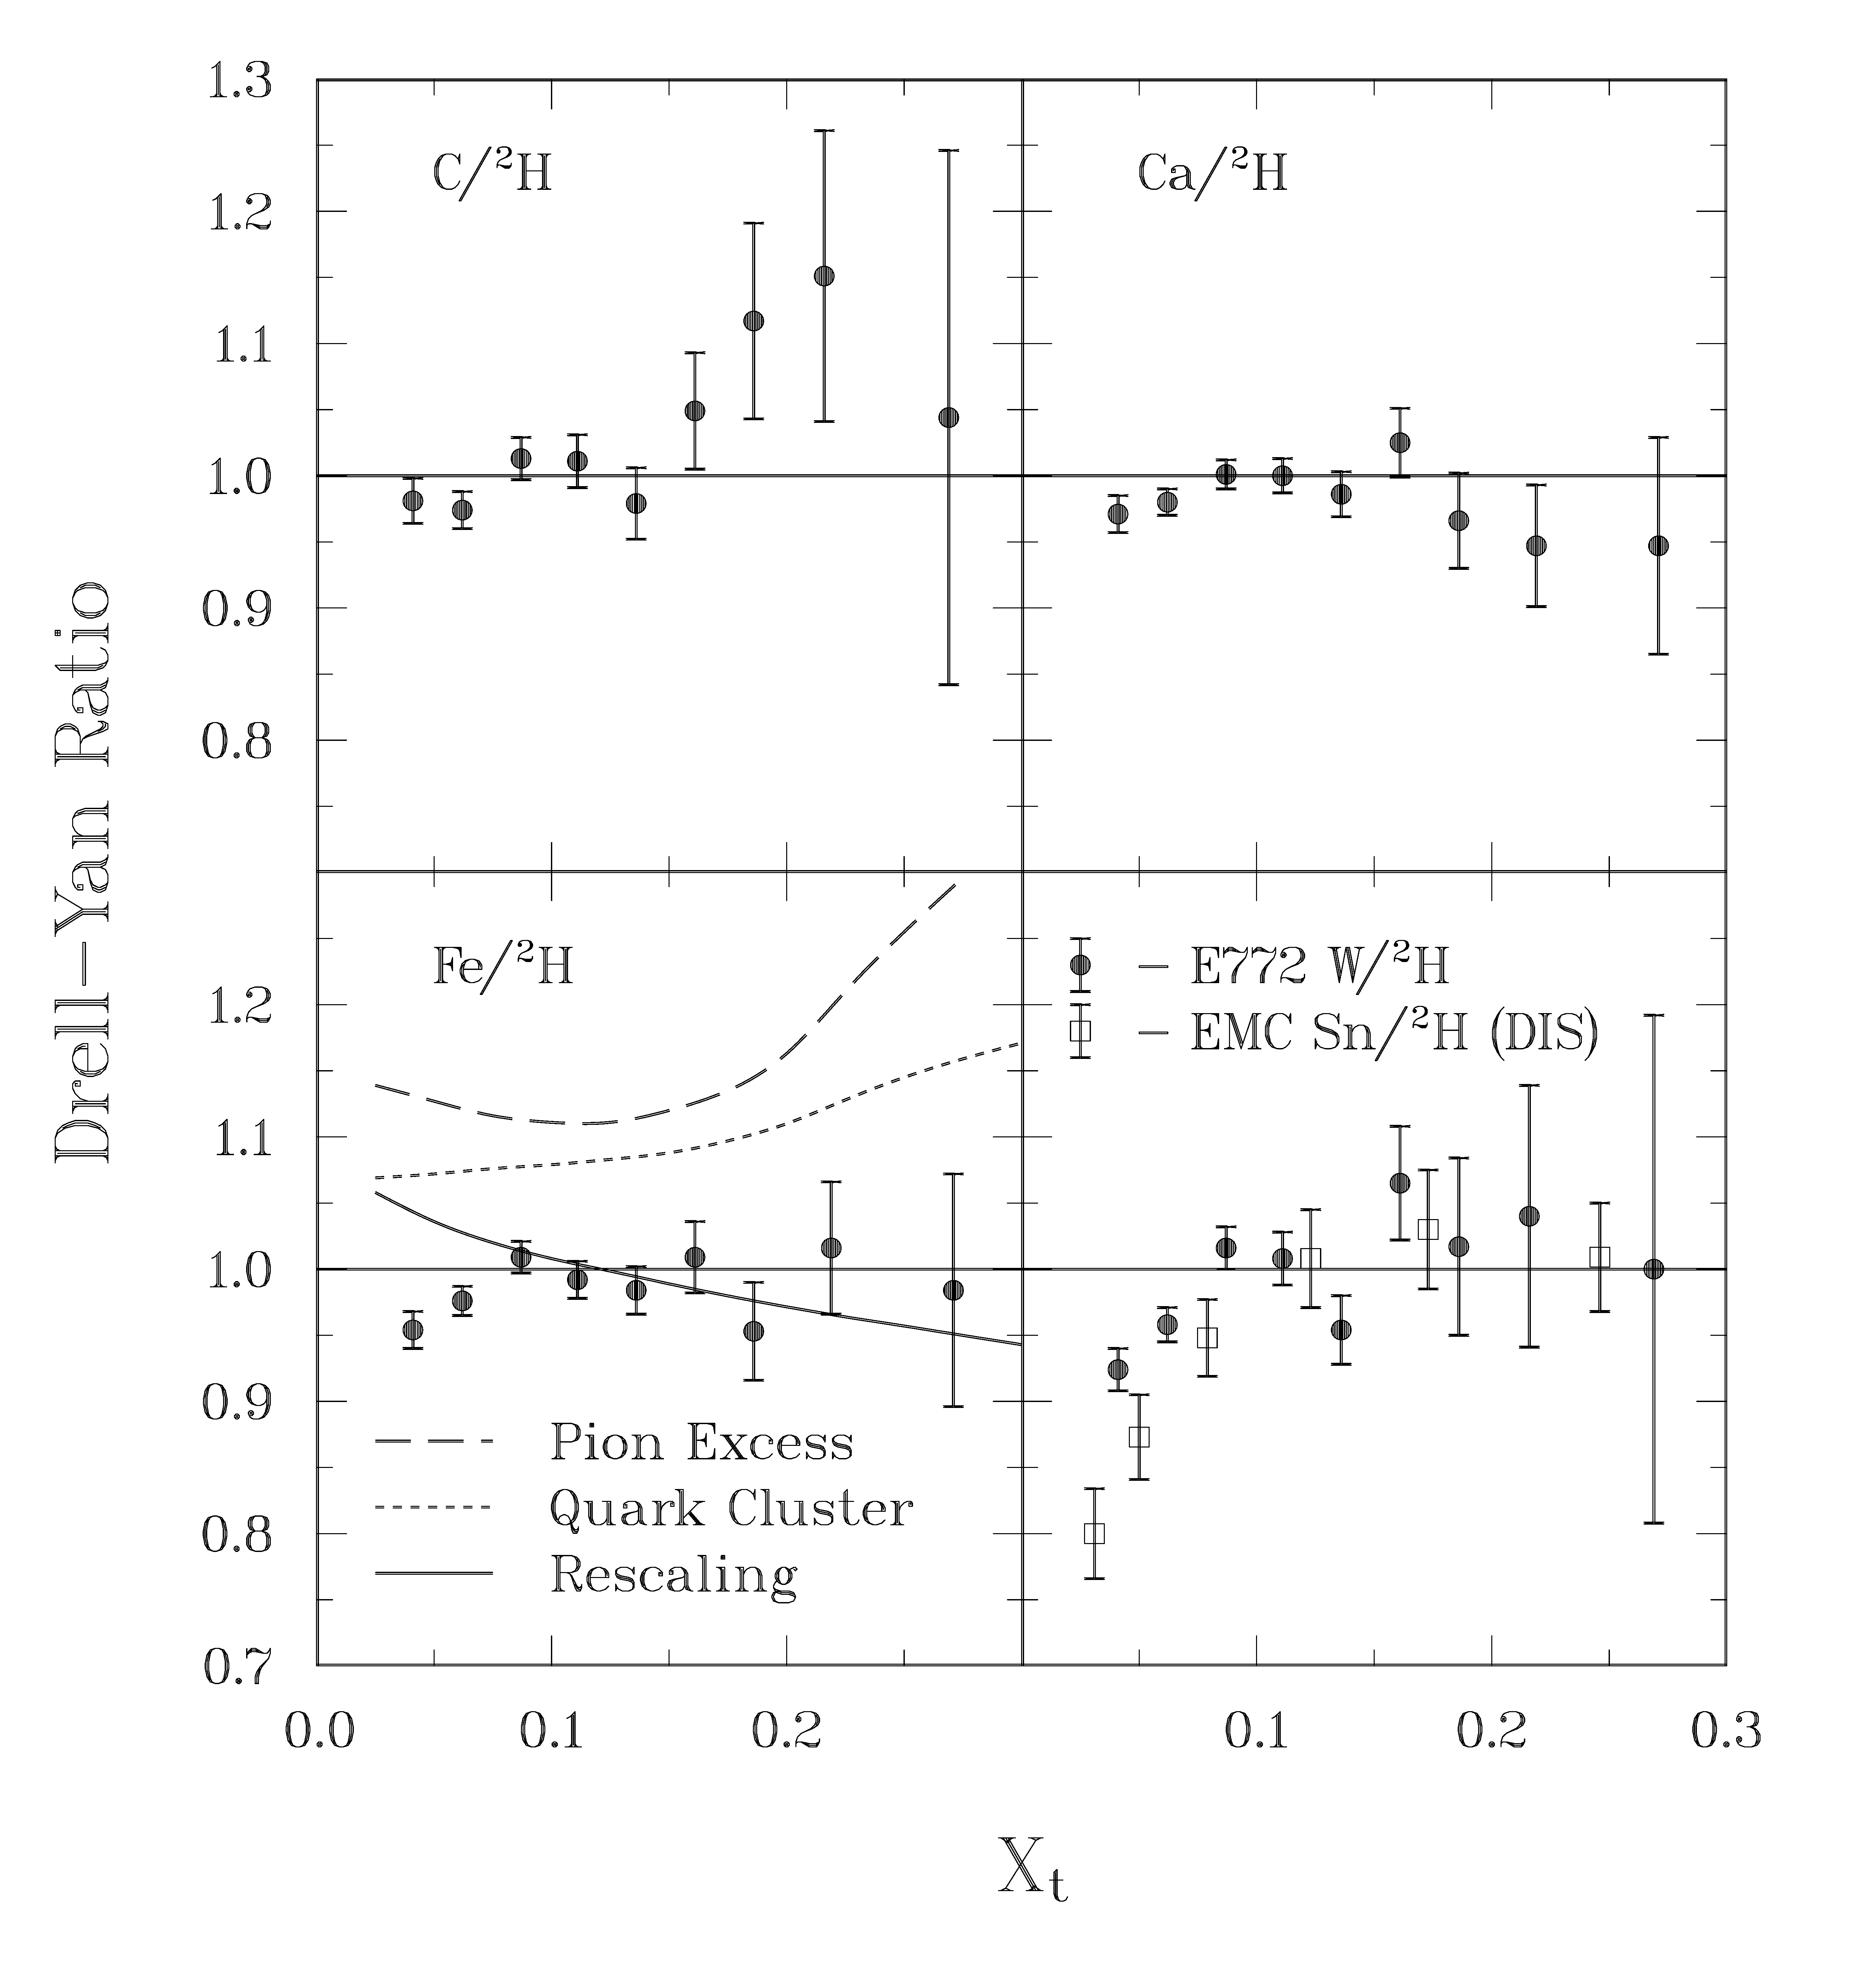
\includegraphics[width=\textwidth]{figures/background/dyfig9.png}
	\caption{The slopes of the EMC ratio for $0.35<x<0.7$ vs the average nuclear density scaled by $(A-1)/A$~\cite{Seely:2009gt}.}
	\label{fig:emc-slope-vs-density}
\end{figure}

\subsection{$x>1$ Plateaus in EMC Ratio}

What has recently spurred renewed interest in the EMC effect and its possible true origin is a series of measurements by JLAB of election DIS cross section ratios where $x>1$. In this kinematic space, the cross section from a free nucleon vanishes, but persists for the deuteron. It may not at first make sense that measurements can be made in this high $x$, but it is accessible. Such a behavior is interpreted as the manifestation of short-range nucleon-nucleon correlations (three-nucleon correlations for $x>2$). These short range correlations happen when two (or three) nucleons happen to get very close to each other and experience a large repulsive Coulomb force, resulting in the nucleons moving apart from each other with high \emph{individual} momentum, but low \emph{combined} momentum.

\begin{figure}[!tbp]
	\centering
	\begin{minipage}[b]{.4\textwidth}
		\centering
		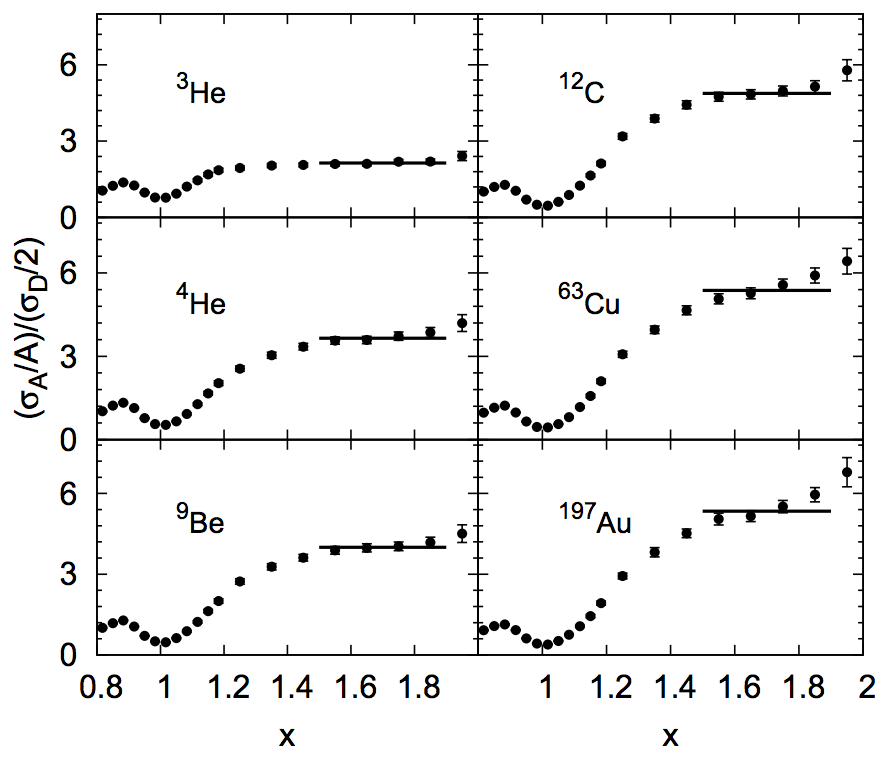
\includegraphics[height=0.3\textheight]{figures/background/nn-src-plateau.png}
		\caption{Per nucleon cross section ratios vs $x$ at $0.8<x<2$ as measured by JLAB-E02019 with a line fit to the ``plateau'' regions at $1.5<x<1.9$~\cite{Fomin:2011ng}.}
		\label{fig:nn-src-plateau}
	\end{minipage}%
	\hfill
	\begin{minipage}[b]{.4\textwidth}
		\centering
		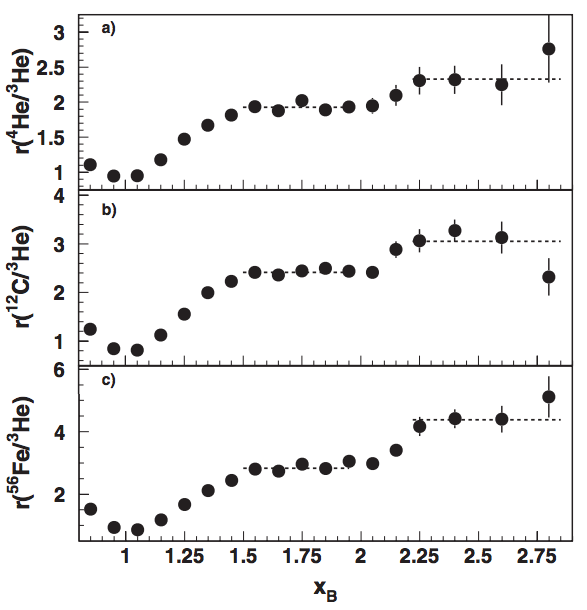
\includegraphics[height=0.3\textheight]{figures/background/CLAS-nnn-src-ratio.png}
		\caption{Per nucleon cross section ratios vs $x$ at $0.75<x<3$ as measured by CLAS with a line fit to the ``plateau'' regions  at $2.25<x<2.8$ \cite{PhysRevLett.96.082501}.}
		\label{fig:nnn-src-plateau}
	\end{minipage}
\end{figure}

The JLAB-E02019 experiment~\cite{Fomin:2011ng} measured cross section ratios for $^3He$, $^4He$, $Be$, $C$, $Cu$ and $Au$ to deuterium. One can see in the results shown in Figure~\ref{fig:nn-src-plateau} that the cross section ratios of $^4He/D$, $C/D$ and $Cu/D$ rise with $x$ until the value plateaus at $x \approx 1.4 - 1.5$. The key observation with these plateaus is that the ratio value at this plateau increases with $A$. Such behavior was already observed with less accuracy by an experiment at SLAC~\cite{Frankfurt:1993sp}, and a similar pattern can be seen in the CLAS experiment which compared nuclear cross sections to tritium ($^3He$)~\cite{PhysRevLett.96.082501}. Here the measurements extend up to $x=3$ and an indication of a second plateau is observed for $2.25<x<2.8$ (Fig.~\ref{fig:nnn-src-plateau}). The variable $a_2(A/d)$, also called the Short Range Correlation (SRC) Scale Factor\footnote{More specifically, it is called the 2N-SRC scale factor, as there is a three nucleon scale factor for cross section ratios with respect to tritium.} is introduced here as the ratio plateau values in this first plateau range. The variables $a_2(A/^3He)$ and $a_3(A/^3He)$ is also defined for first and second plateau ranges, respectively, but are not used here.



%Fig. 9 shows a very interesting observation [36]. In the left panel the E139 cross section ratios 4He/D, C/D and Fe/D are shown for x < 1. The lines correspond to the slopes d(σA/σD)/dx in the region 0.35 ≤ x ≤ 0.7, that characterize the strength of the EMC effect in this region and are unaffected by overall normalization uncertainties. In the middle panel the slopes of the E139 data (tabulated in [36] and corrected by xA = xp · AMp/MA [49]) are plotted against the height of the plateaus [33]. Obviously there is a strong correlation between these quantities as indicated by the straight line. It is rather unlikely that this correlation is purely accidental and one can therefore rather safely assume that a large fraction of the strength of the EMC effect in the valence quark region is due to short-range nucleon-nucleon correlations.

\subsection{Models For the EMC Effect}

\subsubsection{Pion Cloud Model}

\subsubsection{Rescaling}

\subsubsection{Nuclei-Nuclei Short Range Correlations}

\subsection{The Role of Drell-Yan in Studying the Quark Sea and EMC }

There have been many models attempting to explain the $A$-dependence of such phenomena as the EMC effect. Each of these models provide a prediction regarding the individual sea/valence quark/antiquark distribution functions. In order to test these predictions, one can take stock of the many nuclear probes and assess the capabilities of what each can contribute.

In general, since deep inelastic scattering of electrons and muons is an electromagnetic interaction, it is not innately sensitive to the whether or not the struck quark was a valence quark or a sea quark and can only measure the charge-weighted (E\&M+weak) sum of parton distributions. Through neutrino and antineutrino DIS it is possible to discern between valence and sea distributions. It is the case that most models make predictions for valence quark distributions at mid-to-high $x$ that are not in tension with each other. As such, measuring the valence distributions would not help much in discriminating between different models. Models do, however, differ in their predictions on the sea quark distributions at higher x ($x\gtrsim0.2$) - but at high momentum fraction, the distributions of sea quarks diminish very quickly (Fig.~\ref{fig:pdf-q2-q100}). As such, obtaining precision measurements from antineutrino DIS has been unable to deliver precise measurements of sea quark distributions at high-$x$ yet.

The Drell-Yan process, $pA\rightarrow l^+l^-$, uses the $s$-channel version of the same DIS process, but due to the nature of requiring interacting $q\bar{q}$ pairs, it provides a tool that allows one to cleanly and specifically investigate the sea quark distributions. With a forward spectrometer (such as is the case for E-772 and SeaQuest), where one accepts the $x_F>0.1$ one is able to study the Drell-Yan interaction in the specific case of a valence quark from a free proton (the beam) annihilating with an antiquark from the quark sea in the target. As a result, a study of this process for various nuclei can provide a direct, precise measurement of the $\ubar$, and thereby sea quark distributions that can assist in evaluating the plethora of EMC effect models out there, along with refining constraints on global fits of PDFs.

In this paper, the A-dependence of the Drell-Yan cross sections is studied, which directly measures the A-dependence of the antiquark distributions~\cite{Berger:1985dr}. We define this ratio, $R^{DY}$ as the ratio of Drell-Yan differential cross-sections, using Eq.~\ref{eq:DY-cross} to get
\begin{eqnarray}
	R^{DY} & \equiv & \frac{d^2\sigma_A}{dx_1 dx_2} \Biggm/ \frac{d^2\sigma_d}{dx_1 dx_2} \\
	 & \approx & \frac{\sum_f e_f^2 \cdot q_f^{\text{beam}}(x_1) \bar{q}_f^A(x_2)}{\sum_f e_f^2 \cdot q_f^{\text{beam}}(x_1) \bar{q}_f^d(x_2)}.
\end{eqnarray}
Assuming that the $\ubar$ distribution is roughly similar to the $\dbar$ distribution in the target, this term is dominated by up-quark contributions by a factor of eight: $e_u^2 = 4 e_d^2$, and there are twice as many up-quarks from the beam proton as down quarks~\cite{Geesaman:1995yd}. As a result, we can approximate
\begin{eqnarray}
	R^{DY} & \approx & \frac{e_u^2 \cdot q_u^{\text{beam}}(x_1) \bar{q}^A_u(x_2)}{e_u^2 \cdot q_u^{\text{beam}}(x_1) \bar{q}^d_u(x_2)} \\ 
	& = & \frac{\bar{q}_u^A(x_2)}{\bar{q}_u^d(x_2)}
\end{eqnarray}
meaning that by measuring $R^{DY}$ for $pA$ to $pd$ collisions with a forward spectrometer, a good measure of the nuclear modification of the anti up quark sea distributions can be achieved.

\subsubsection{Previous Measurements}

\begin{wrapfigure}{r}{0pt}
\centering
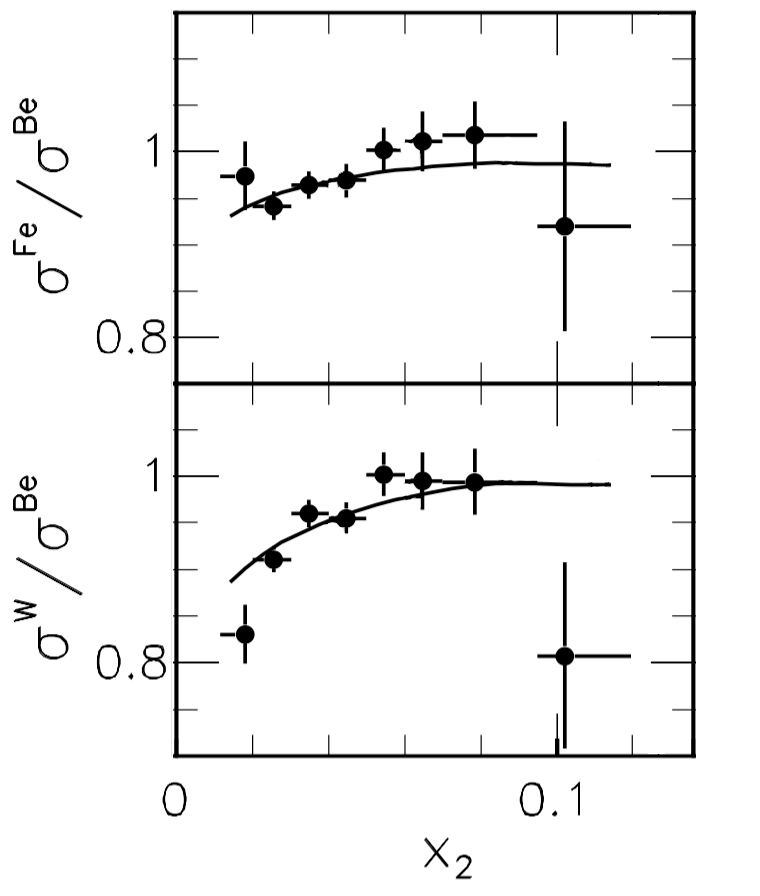
\includegraphics[width=0.35\textwidth]{figures/background/e866-emc-ratio.png}
\caption{E-866 Drell-Yan $\sigma^A/\sigma^{Be}$ for iron and tungsten as a function of $x_2$~\cite{Vasilev:1999fa}.}
\label{fig:866-emc}
\end{wrapfigure}
Even though Drell-Yan events for $x_1>0.3$ do directly measure the sea quark distribution, there is a limited amount of data available.

\begin{figure}[h]
	\centering
	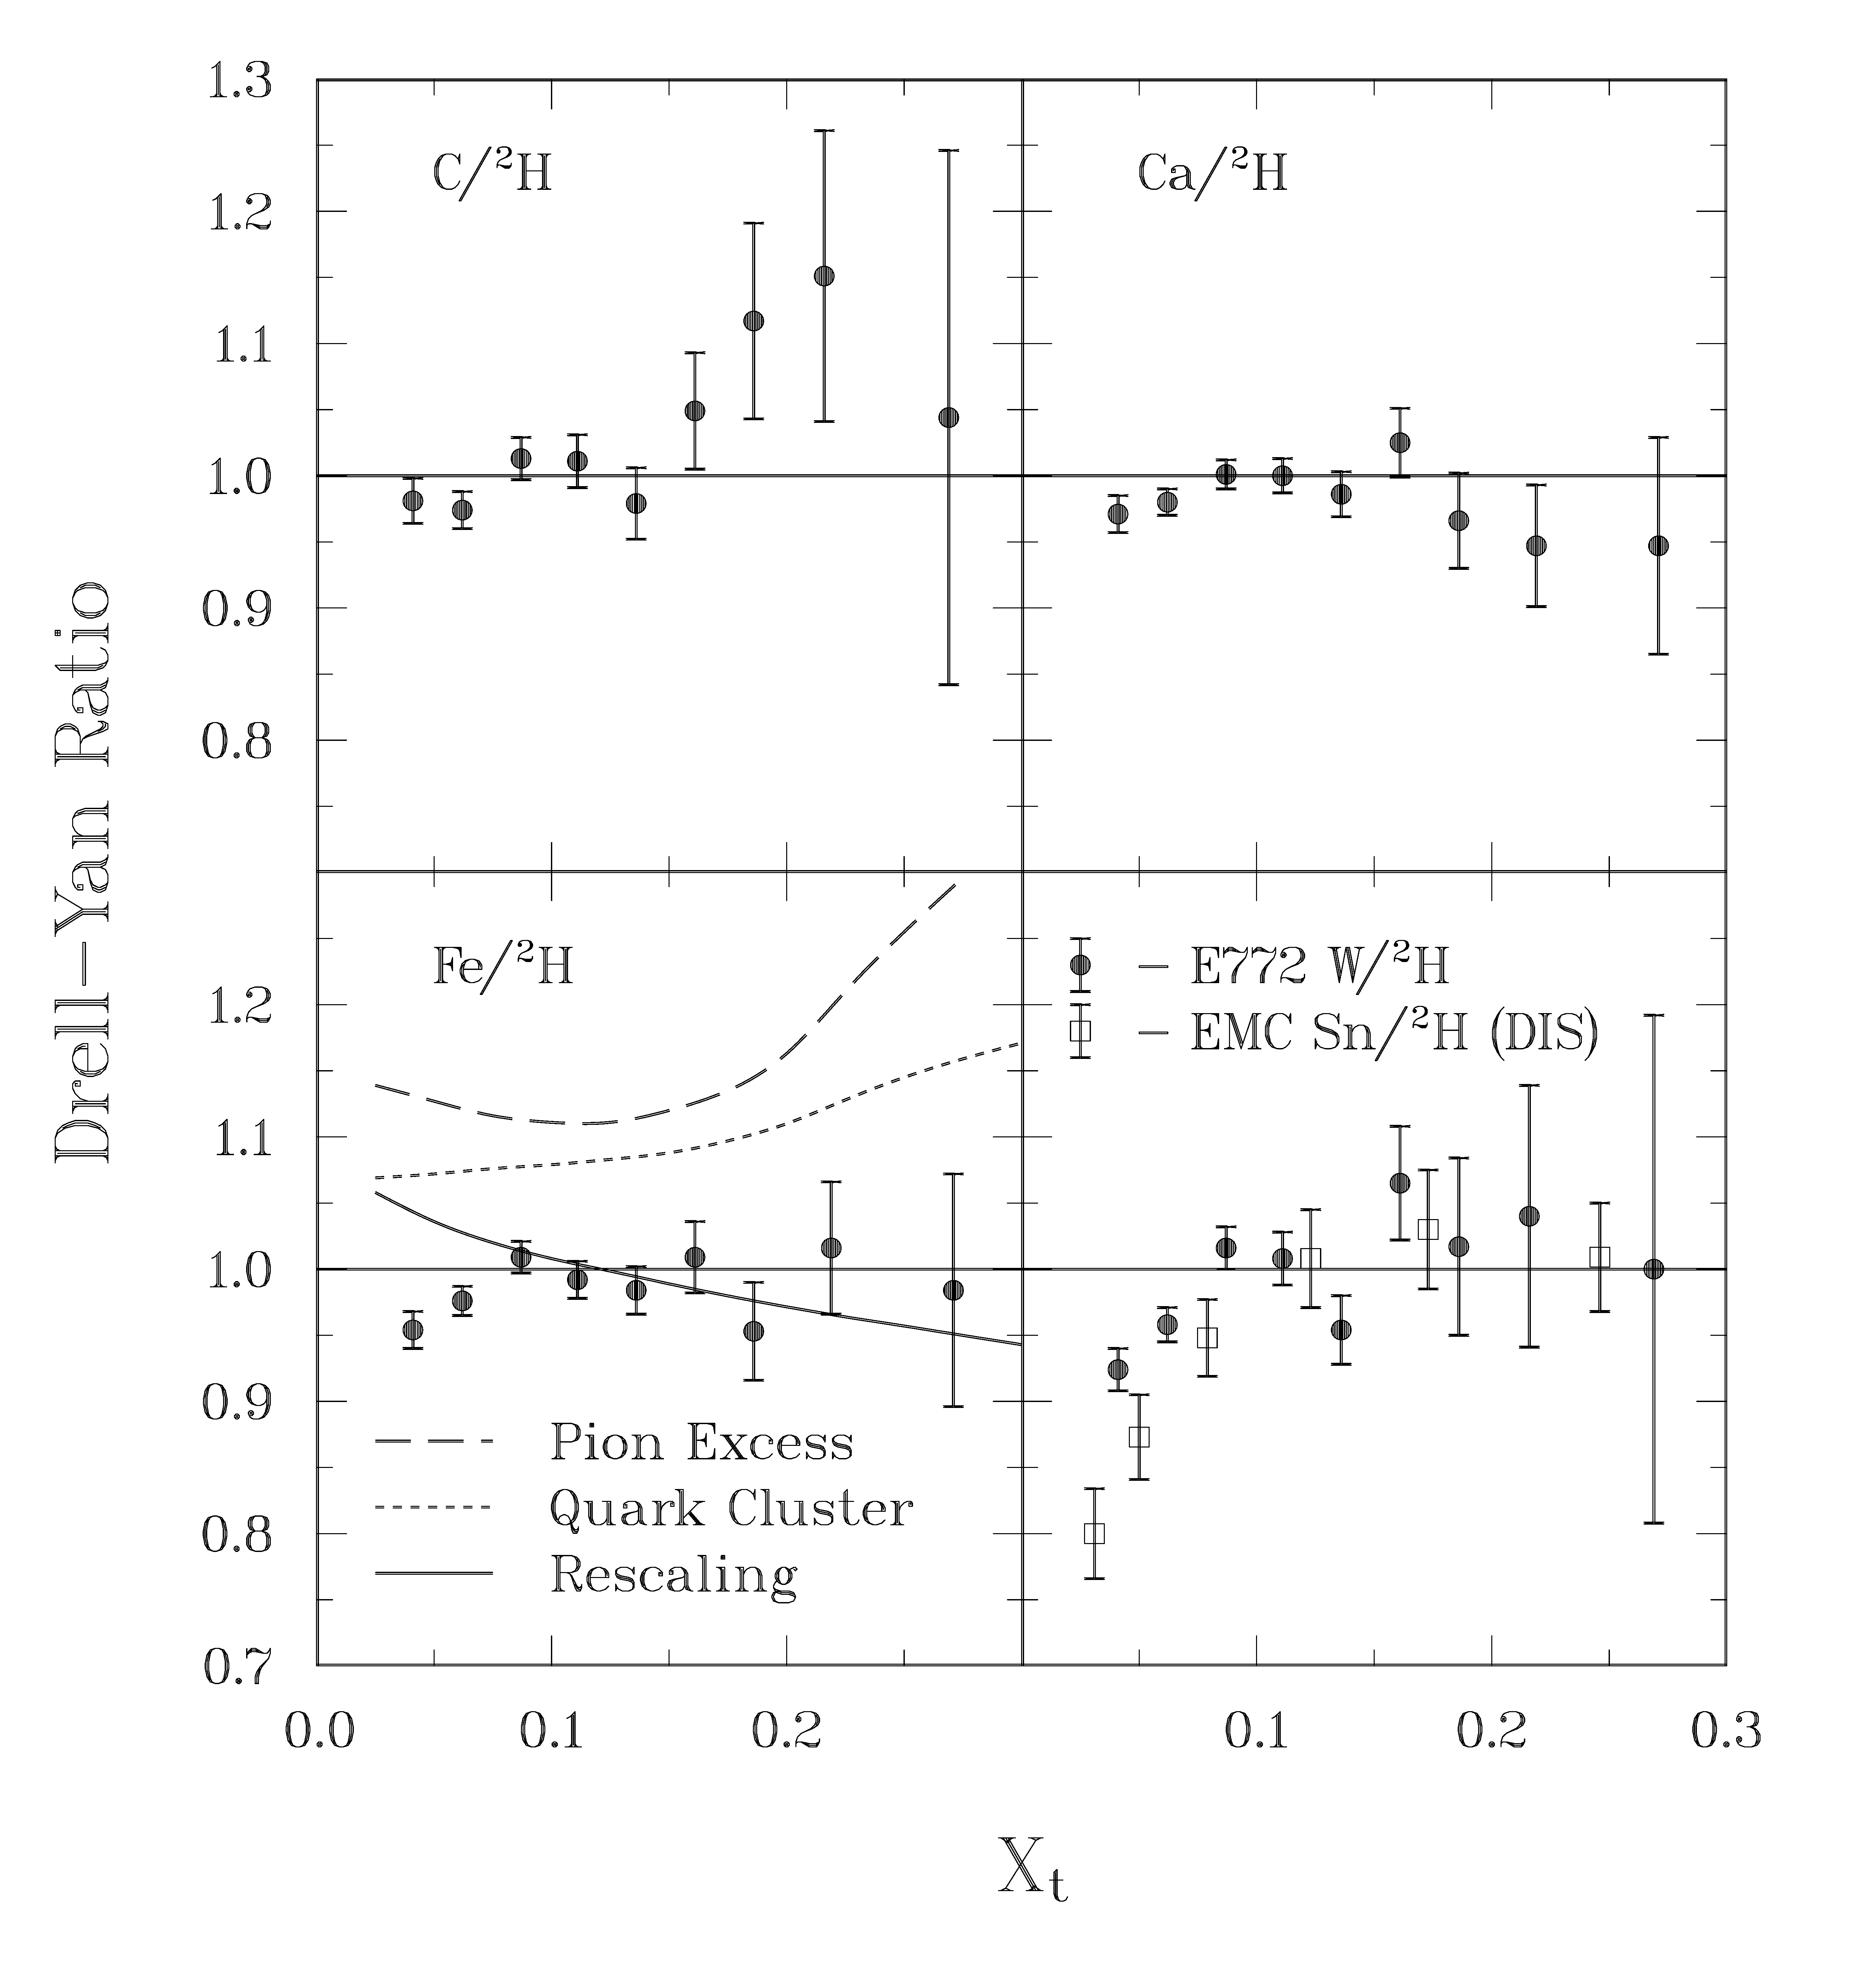
\includegraphics[width=\textwidth]{figures/background/dyfig9.png}
	\caption{E-772 Drell-Yan $\frac{A}{^2H}$ ratios for several nuclear targets as a function of $x_2$ ($x_t$)\cite{Alde:1990im}.}
	\label{fig:772-dy}
\end{figure}

\subsection{Nuclear Dependence of Drell-Yan at SeaQuest}

\red{\begin{itemize}
		\item Talk about what will be measured
		\item Which targets will be used
		\item What kinematic phase space in \{x1, x2\} will be explored
		\item What the statistics will be, approximately
		\item What, if anything, will be compared to models
	\end{itemize}}


%Recent experiments at Hall C at JLab and SLAC suggest the following regarding the EMC Effect \cite{Seely:2009gt}:
%\begin{itemize}
%	\item
%	It is $Q^2$-independent.
%	\item
%	It's x-dependent shape is universal (across various nuclei).
%	\item
%	The magnitude (slope) of the effect varies with A.
%	\item
%	There is a ``shadowing'' effect at very low-$x$.
%	\item
%	Fermi motion dominates the ratio at high-$x$.
%\end{itemize}